% !TEX program = pdflatex
% !TEX enableSynctex = true
\documentclass[aspectratio=169,10pt]{beamer}

%%%%%%%%%%%%%%%
\usepackage{booktabs}
\usepackage{xspace}
\usepackage{ulem}
\usepackage{subfig}
\usepackage{graphicx}
\usepackage{xcolor}
\usepackage{multirow}
\usepackage[capitalise,noabbrev]{cleveref}
\usepackage{datatool}
\usepackage{algorithm}
\usepackage{algpseudocode}
\usepackage{empheq}
\usepackage[many]{tcolorbox}
\usepackage{amssymb}
\usepackage{dsfont}
\usetheme[progressbar=frametitle,block=fill]{metropolis}

\newcommand{\themename}{\textbf{\textsc{metropolis}}\xspace}
\usefonttheme{professionalfonts}
\definecolor{KahouBlack}{RGB}{31, 28, 26}
\definecolor{KahouGold}{RGB}{201, 168, 76}
\definecolor{KahouLightGold}{RGB}{240, 225, 180}
\definecolor{emphcolorval}{RGB}{128, 0, 32}
\definecolor{highlightcolorval}{rgb}{1,0,0}
\definecolor{Terracotta}{RGB}{180, 90, 60}
\definecolor{TerracottaLight}{RGB}{242, 236, 220}
\definecolor{Sienna}{RGB}{120, 55, 25}
\definecolor{SlideBackground}{RGB}{252, 249, 240}
\tcbset{lossbox/.style={
  enhanced, colback=TerracottaLight, colframe=Terracotta,
  boxrule=1pt, arc=3pt, left=4pt, right=4pt, top=2pt, bottom=2pt,
  before={}, after={}, before upper={\vspace{-2pt}}
}}
\tcbset{highlight math style={
  enhanced, colback=TerracottaLight, colframe=Terracotta,
  boxrule=1pt, arc=3pt, left=4pt, right=4pt, top=2pt, bottom=2pt
}}
\setbeamercolor{frametitle}{bg=KahouLightGold, fg=KahouBlack}
\setbeamercolor{progress bar}{fg=KahouBlack}
\setbeamercolor{math text}{fg=Sienna}
\setbeamercolor{block title}{fg=white, bg=Terracotta}
\setbeamercolor{block body}{fg=KahouBlack, bg=TerracottaLight}
\setbeamercolor{background canvas}{bg=SlideBackground}
\setbeamercolor{button}{fg=KahouBlack, bg=KahouGold}

\setbeamersize{text margin left=5.5pt, text margin right=5.5pt}

\newcommand{\emphcolor}[1]{\textbf{\textcolor{emphcolorval}{#1}}}
\newcommand{\highlightcolor}[1]{{\textbf{\color{highlightcolorval}{#1}}}}

\crefname{equation}{}{}
\newtheorem{proposition}{Proposition}
\newcommand\bigzero{\makebox(0,0){\text{\huge0}}}
\newcommand{\D}[1][]{\ensuremath{\boldsymbol{\partial}_{#1}}}
\newcommand{\R}{\ensuremath{\mathbb{R}}}
\newcommand{\diff}{\ensuremath{\mathrm{d}}}
\newcommand{\set}[1]{\ensuremath{\left\{{#1}\right\}}}
\newcommand{\indicator}[1]{\ensuremath{\mathds{1}\left\{{#1}\right\}}}
\newcommand{\expec}[2][]{\ensuremath{\mathbb{E}_{{#1}}\left[ {#2} \right]}}
\newcommand{\bigO}[1]{\ensuremath{\mathcal{O}(#1)}}
\newcommand{\Xdom}{\mathcal{X}}
\newcommand{\Yrange}{\mathcal{Y}}
\newcommand{\Xtrain}{\mathcal{X}_{\mathrm{train}}}
\newcommand{\Xtest}{\mathcal{X}_{\mathrm{test}}}
\newcommand{\F}{\mathcal{F}}
\newcommand{\Resid}{\mathcal{R}}
\newcommand{\Op}{\mathcal{T}}
\newcommand{\st}{\textrm{s.t.}\,}

\begin{document}
\title{{\vspace{0.4in}\hspace{0.2in}\textcolor{KahouBlack}{The Blessings of Overparameterization: \\ \hspace*{5mm}Applications in Solving Economic Models}}}
\author{\hspace*{4mm} Mahdi Ebrahimi Kahou\inst{1} \and
	Jes\'{u}s Fern\'{a}ndez-Villaverde\inst{2}}

\institute{\inst{1}Bowdoin College \and
	\inst{2}University of Pennsylvania}

\date{}

\maketitle

\section{\textcolor{KahouBlack}{Motivation, Question, and Contribution}}

\begin{frame}{Motivation}
	\begin{center}
		\emphcolor{``I remember my friend Johnny von Neumann used to say, with four parameters I can fit an elephant, and with five I can make him wiggle his trunk.''---{\it Enrico Fermi}}
		\vspace{0.1in}
	\end{center}
	\vspace{0.1in}
	\begin{itemize}
		\item Deep learning has proved remarkably capable at solving \emphcolor{high-dimensional problems}.
		\vspace{0.1in}
		\item Economists are now using it to find accurate approximate solutions to dynamic models once thought intractable.
		\vspace{0.1in}
		\item These networks are \emphcolor{massively overparameterized}, with far more parameters than ``data'' points.
		\vspace{0.1in}
		\item Standard statistical wisdom says: more parameters than ``data'' points leads to \emphcolor{overfitting} and poor out-of-grid performance.
	\end{itemize}
\end{frame}

\begin{frame}{Question}
	When solving dynamic models with neural networks
	\begin{itemize}
		\item Does overparameterization lead to poor approximation in out-of-grid performance?
		\vspace{0.1in}
		\item Is overparameterization a ``necessary evil'' that comes with modern machine learning methods, or does it give us something extra?
		
	\end{itemize}
\end{frame}

\begin{frame}{Contribution}
	\begin{enumerate}
		\item \emphcolor{No overfitting:} as the number of network parameters grows, the solutions become more accurate.
		\vspace{0.1in}
		\item \emphcolor{Algorithmic stability:} the approximate solutions of dynamic models in economics are unstable; overparameterization increases stability.
	\end{enumerate}
	\begin{block}{Implication}
		When in doubt, use a bigger network. Overparameterization is not a source of risk to be managed but a feature to be exploited.
	\end{block}
\end{frame}

%=====================================================================
\section{\textcolor{KahouBlack}{Background: Economic Models, Approximate Solutions, and Overparameterization}}
%=====================================================================

\subsection{\textcolor{KahouBlack}{What do we mean by ``solving a model''?}}


\begin{frame}{An economic model is a system of functional equations}
	Many theoretical models can be written as functional equations:
	\begin{itemize}
		\item Economic object of interest: $f $, where $f : \Xdom\to \mathcal{R}\subseteq \mathbb{R}^N$ 
		\begin{itemize}
			\item e.g., production, investment choice, best-response, etc.
		\end{itemize}
		\vspace{0.1in}
		\item Domain of $f$: $\Xdom$  
		\begin{itemize}
			\item e.g. space of capital, opponents state, etc.
		\end{itemize}
		\vspace{0.1in}
		\item The ``Economics model'':  $\ell \big(x,f\big)$  
		\begin{itemize}
			\item e.g., Euler and Bellman residuals, equilibrium FOCs.
		\end{itemize}
		\vspace{0.1in}
	\end{itemize}
	Then a \emphcolor{solution} is $f^*\in \F$ where $\ell(x,f^*) = \mathbf{0}$ for all $x \in \Xdom$.\vspace{0.1in}
\end{frame}

\begin{frame}{Approximate solution}
	\begin{enumerate}
		\item Sample $\mathcal{X}$: $\mathcal{D} = \{x_1,\cdots,x_N\}$
		\vspace{0.025in}
		\item Pick a family of parametric functions (e.g., polynomials, Chebyshev polynomials, neural networks) $f_\theta(\cdot)$:
		\begin{itemize}
			\item $\theta = \{\theta_1,\cdots,\theta_M\}$: parameters for optimization (e.g., coefficients, or weights and biases).
		\end{itemize}
		\vspace{0.025in}
		\item To find an approximation for $f$ solve:
		\begin{align*}
			\min_{\theta } \frac{1}{N}\sum_{x \in \mathcal{D}} \|\underbrace{\ell(x,f_\theta)}_{\text{Econ model error}}\|_2^2
		\end{align*}
	\end{enumerate}
\end{frame}

\begin{frame}{Neural Networks and Overparameterization}
	\emphcolor{Neural Networks} form a \emphcolor{highly-overparameterized} ($M\gg N$) class of functions.
	\begin{itemize}

		\item Example: one layer neural network, $f_{\theta} : \mathbb{R}^Q\rightarrow \mathbb{R}$:
		\begin{equation*}
			f_{\theta}(x) = W_2 \cdot \sigma \left(W_1\cdot x+b_1\right)+b_2
		\end{equation*}
		\vspace{0.1in}
		\item $W_1\in \mathbb{R}^{P\times Q}$, $b_1\in \mathbb{R}^{P\times 1}$, $W_2 \in \mathbb{R}^{1\times P}$, and $b_2 \in \mathbb{R}$.
		\vspace{0.1in}
		\item $\theta \equiv \{b_1,W_1,b_2,W_2\}$ are the coefficients, in this example $M = PQ+P+P+1$.
		\vspace{0.1in}
		\item $\sigma(\cdot)$ is a nonlinear function applied element-wise (e.g., $\max\{\cdot,0\}$).
		\vspace{0.1in}
		\item Making it ``deeper'' by adding another ``layer'':
		$f_{\theta}(x)\equiv W_3\cdot\sigma(W_2 \cdot \sigma(W_1 \cdot x + b_1) + b_2)+b_3.$
	\end{itemize}
\end{frame}

\section{\textcolor{KahouBlack}{Applications}}

\begin{frame}{Experimental design}
	\begin{itemize}
		\item We demonstrate these properties across three canonical models with known benchmarks:
	\end{itemize}
	\vspace{0.1in}
	\begin{columns}
		\begin{column}{0.32\textwidth}
			\begin{block}{1. Linear-Quadratic}
				Closed-form solution. Sharpest test of approximation error.
			\end{block}
		\end{column}
		\begin{column}{0.32\textwidth}
			\begin{block}{2. McCall Job Search}
				1D state, kink at reservation wage. Non-smooth approximation.
			\end{block}
		\end{column}
		\begin{column}{0.32\textwidth}
			\begin{block}{3. Real Business Cycle}
				2D stochastic state. No closed form. Benchmarked vs.\ VFI.
			\end{block}
		\end{column}
	\end{columns}
	\vspace{0.15in}
	\begin{itemize}
		\item In all three: \emphcolor{accuracy} and \emphcolor{stability} improve with overparameterization.
	\end{itemize}
\end{frame}





%\begin{frame}{Contrast with perturbation methods}
%	\begin{itemize}
%		\item A central challenge in solving nonlinear models by perturbation: higher-order Taylor expansions generate explosive sample paths.
%		\item Standard fix: \emphcolor{pruning} (\textcolor{emphcolorval}{Kim et al., 2008; Andreasen et al., 2018}). Cross-products of higher-order terms are deliberately dropped to restore stability.
%		\item Pruning is an exercise in deliberate \emph{under}-parameterization: parameters are removed to make the approximation well-behaved.
%		\item Our paper delivers the \emphcolor{opposite message}: in the neural network approach, \emph{increasing} network width is what delivers accuracy and stability.
%	\end{itemize}
%	\begin{block}{Slogan}
%		The perturbation literature \emph{prunes to survive}; neural network solvers \emph{grow to thrive}.
%	\end{block}
%\end{frame}

%=====================================================================
\section{\textcolor{KahouBlack}{Application 1: Linear-Quadratic regulator}}
%=====================================================================


\begin{frame}{The LQ problem}
	\begin{itemize}
		\item The general deterministic LQ problem:
		\begin{align*}
			v(x) &= \max_u \left\{ -x^\top R\, x - u^\top Q\, u + \beta\, v(x') \right\} \\
			&\st\quad x' = A x + B u, \quad x_0 \text{ given}
		\end{align*}
		\item State variable: $x\in \mathbb{R}^{n}$. Control variable: $u\in \mathbb{R}^k$.
		\item Closed-form solution:
		\begin{empheq}[box=\tcbhighmath]{align*}
			v(x) = -x^\top P x, \qquad u(x) = -F x
		\end{empheq}
		where $P$ and $F$ are obtained from the discrete-time algebraic Riccati equation.
		\item Sharpest test: approximation error can be computed exactly at every point.
	\end{itemize}
\end{frame}

\begin{frame}{A competitive firm with adjustment costs}
	\begin{itemize}
		\item A price-taking firm in a competitive industry.
		\item Own output $y$, aggregate output $Y$ (exogenous). Inverse demand: $\alpha_0 - \alpha_1 Y$.
		\item The firm chooses investment $u$ subject to quadratic adjustment cost $\tfrac{\gamma}{2}u^2$:
		\begin{align*}
			v(y,Y) &= \max_u \left\{ (\alpha_0 - \alpha_1 Y)y - \tfrac{\gamma}{2}u^2 + \beta\, v(y',Y') \right\} \\
			&\st\quad Y' = h_0 + h_1 Y, \quad y' = y + u
		\end{align*}
		\item State is two-dimensional: $(y,Y)$. With augmented state $x = (1, y, Y)^\top$, this maps into the general LQ framework.
		\item Euler equation:
		\begin{empheq}[box=\tcbhighmath]{align*}
			\gamma\, u(y,Y) = \beta\left[\gamma\, u(y',Y') + (\alpha_0 - \alpha_1 Y')\right]
		\end{empheq}
	\end{itemize}
\end{frame}


\begin{frame}[label=lq-nn-impl]{LQ: neural network implementation}
	\begin{itemize}
		\item \emphcolor{Architecture:} one-hidden-layer ReLU networks for value and policy functions. Hidden units $H = 1$ to $H = 7$ (4 to 22 parameters).
		\item \emphcolor{Training data:} the optimal $u$ depends only on $Y$ ($y$ enters linearly and does not affect the marginal return to investment), so we minimize the mean squared Euler residual over $n_Y = 6$ grid points:
		\begin{empheq}[box=\tcbhighmath]{align*}
			\min_{\theta_u} \frac{1}{n_Y} \sum_{i=1}^{n_Y} \left[\gamma\, u(Y_i;\theta_u) - \beta\big(\gamma\, u(Y_i';\theta_u) + \alpha_0 - \alpha_1 Y_i'\big)\right]^2
		\end{empheq}
		\item  Adam optimizer with early stopping at loss $< 10^{-8}$.
		\item \emphcolor{Test data:} $T = 29$ period path simulated from fixed initial conditions. Test points lie in the interior of the state space and never on a training node.
	\end{itemize}
	\vspace{0.05in}
	\hfill\hyperlink{lq-param}{\beamerskipbutton{Parameterization}}
\end{frame}
\begin{frame}{Deep learning is a \emphcolor{non-convex} optimization}
	\begin{itemize}
		\item Deep learning is a non-convex optimization.
		\vspace{0.1in}
		\item In non-convex optimization solutions depends on the initialization of weights and biases $\theta$.
		\vspace{0.1in}
		\item Most economic dynamical models are non-linear.
		\vspace{0.1in} 
		\item We run the algorithm for $50$ different initialization (seed) of the weights and biases.
	\end{itemize}
\end{frame}

\begin{frame}{LQ: train and test Euler-residual loss}
	\begin{figure}[t!]
		\centering
		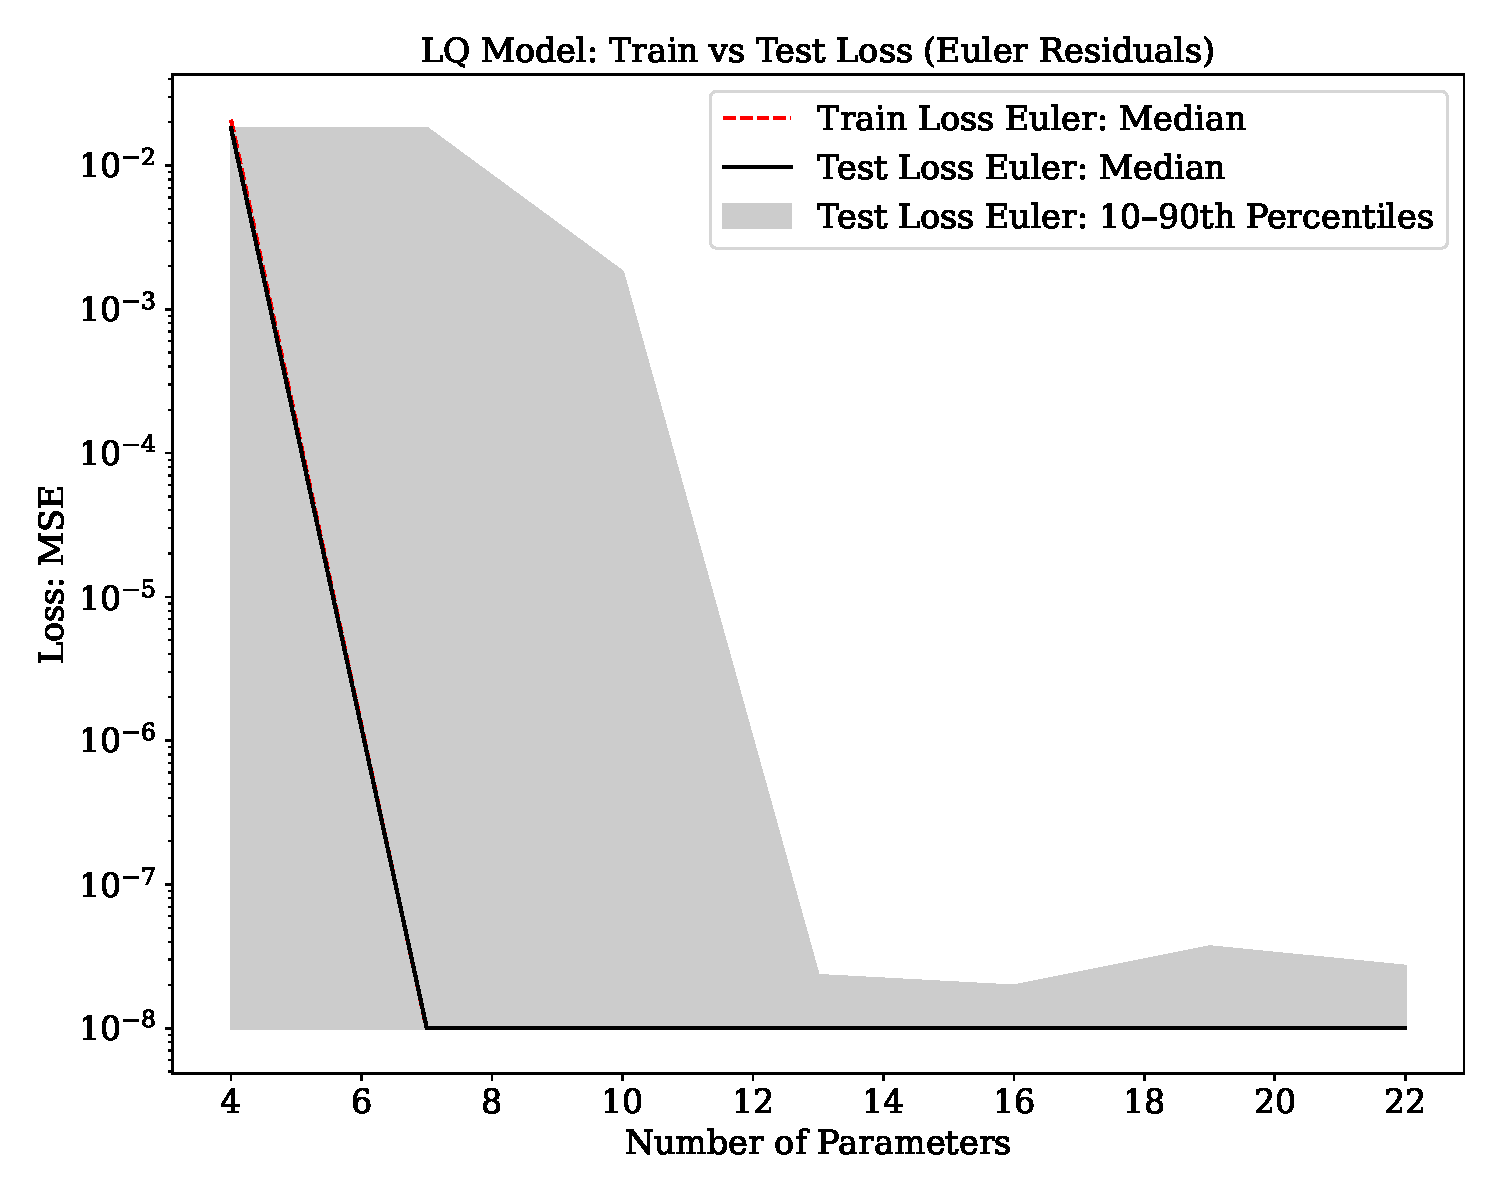
\includegraphics[width=0.62\textwidth]{figures/LQ_policy_test_train_loss.pdf}
	\end{figure}
	\begin{itemize}
		\item Generalization gap is zero throughout: train and test curves are indistinguishable at every width. Direct consequence of the linear structure of the LQ Euler equation.
	\end{itemize}
\end{frame}



\begin{frame}{LQ: absolute relative error vs.\ closed-form solution}
	\begin{figure}[t!]
		\centering
		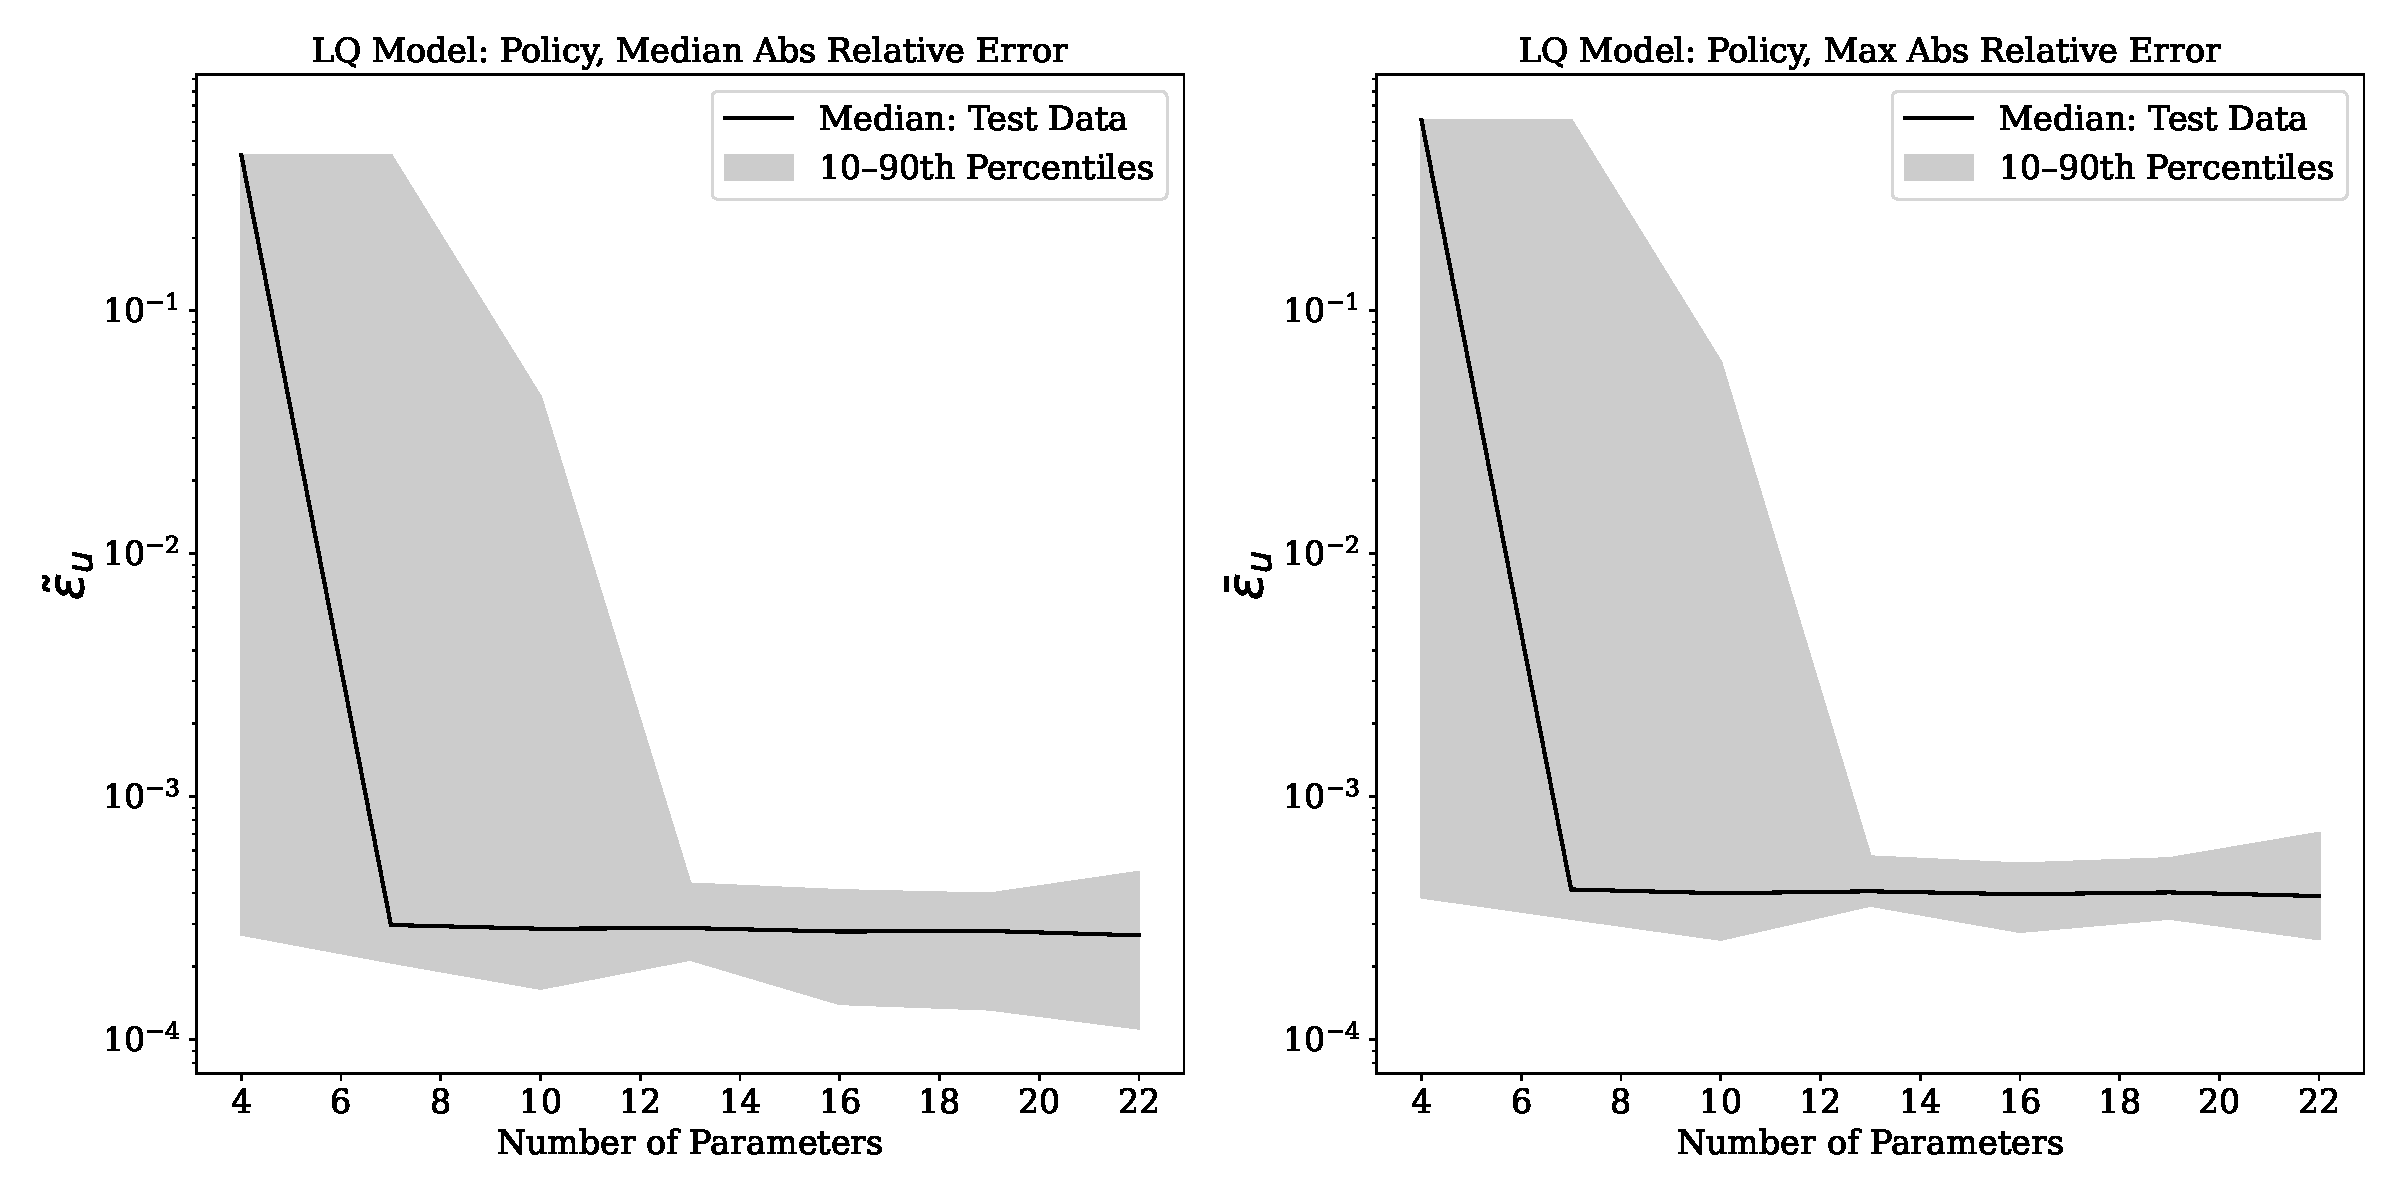
\includegraphics[width=0.8\textwidth]{figures/LQ_policy_rel_error_median_vs_max.pdf}
	\end{figure}
	\begin{itemize}
		\item Median (left) and maximum (right) absolute relative error of the NN policy. Both statistics and their cross-seed dispersion fall with network width.
	\end{itemize}
\end{frame}

\begin{frame}{LQ: policy paths, underparameterized vs.\ overparameterized}
	\begin{figure}[t!]
		\centering
		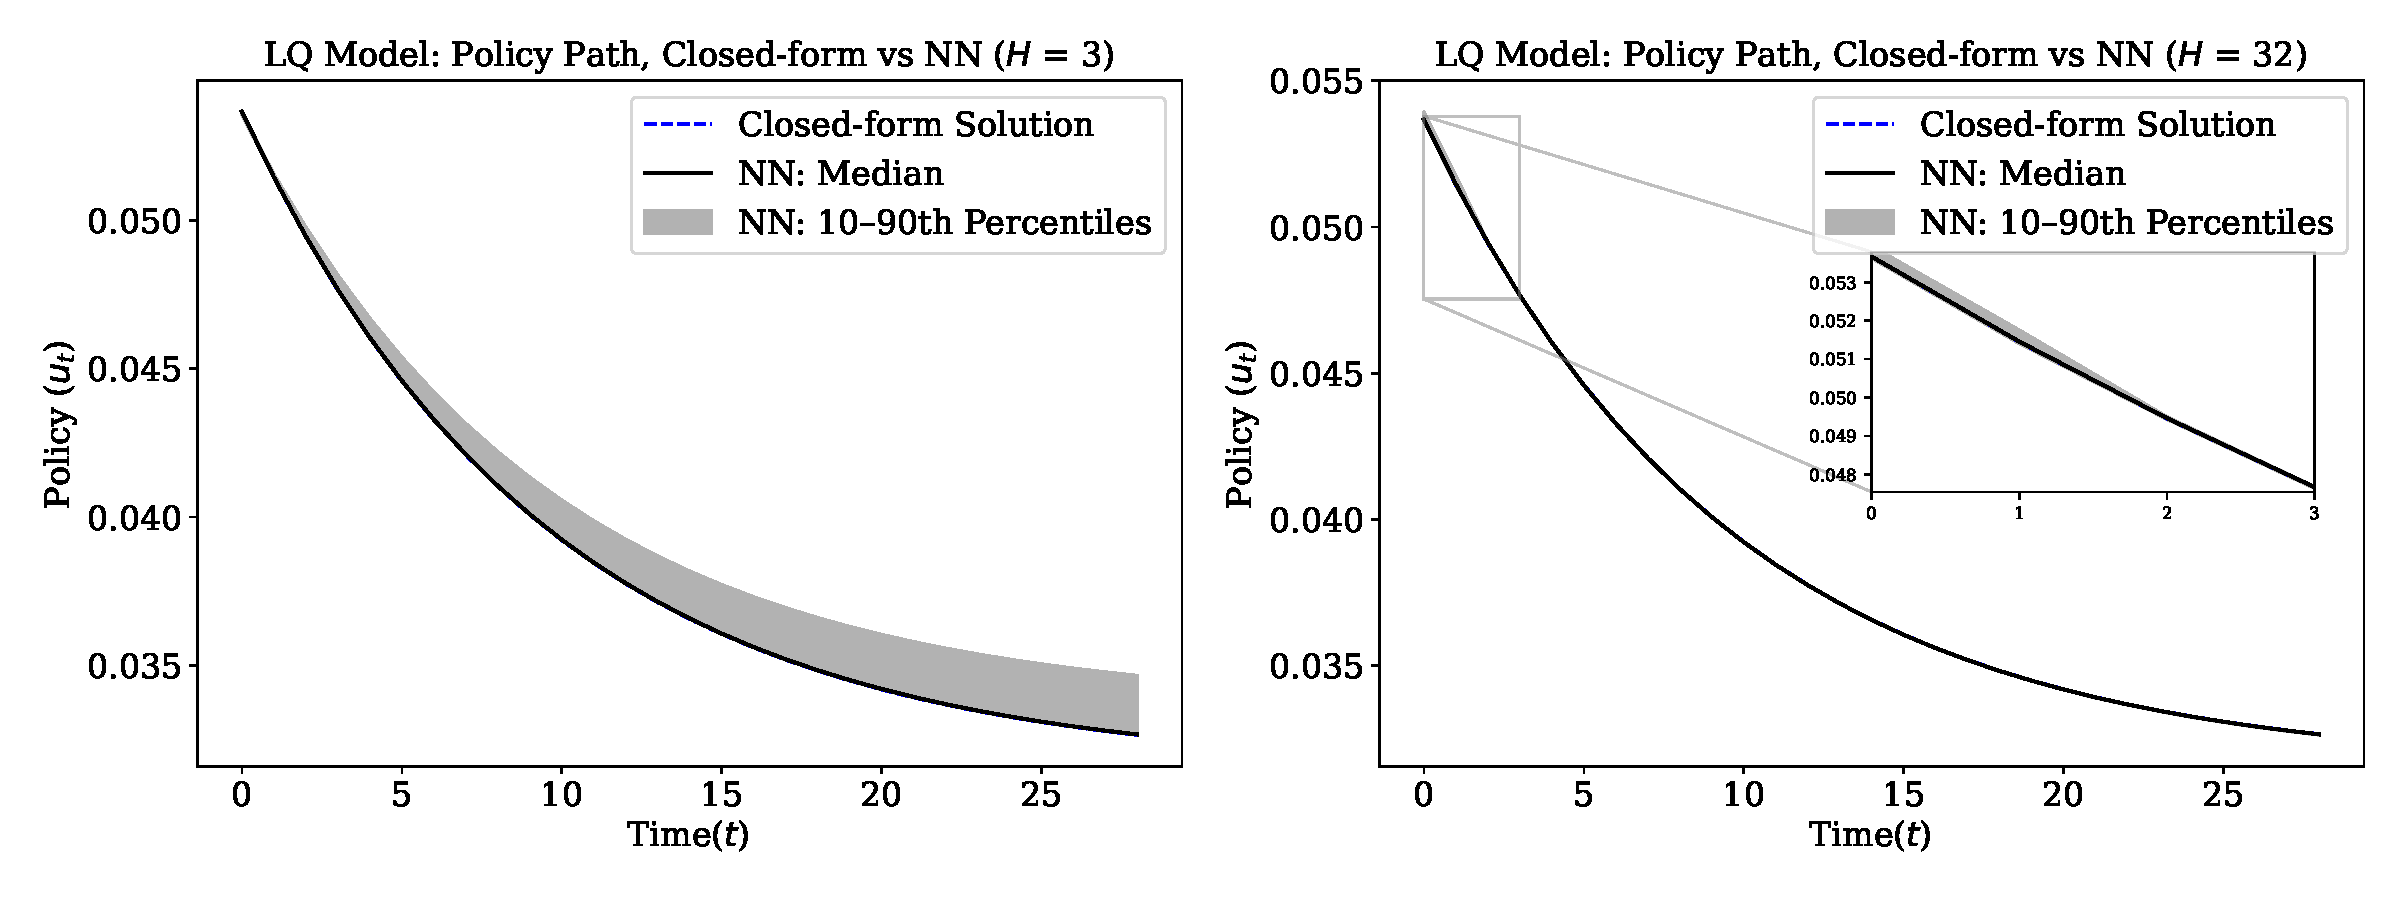
\includegraphics[width=0.85\textwidth]{figures/LQ_policy_path_3_vs_32.pdf}
	\end{figure}
	\begin{itemize}
		\item Left: $H = 3$ (underparameterized). Median is roughly accurate, but the across-seed band is wide.
		\item Right: $H = 32$ (overparameterized). Median tracks the closed-form solution closely \emph{and} the band collapses.
	\end{itemize}
\end{frame}



%=====================================================================
\section{\textcolor{KahouBlack}{Application 2: McCall job-search model}}
%=====================================================================

\begin{frame}{From a linear to a non-smooth problem equation}
	\begin{itemize}
		\item The LQ model is linear, which makes it the cleanest test but also the easiest.
		\item Does the blessing survive when the operator $\Op$ is nonlinear and the solution is non-smooth?
		\item The McCall model (\textcolor{emphcolorval}{McCall, 1970}) provides exactly this test: the value function has a \emphcolor{kink} at the reservation wage, so the network must approximate a non-differentiable function.
		\item An unemployed worker receives i.i.d.\ wage offers $w \sim f$ on $[0,B]$ each period.
		\item Accept: permanent income stream $w/(1-\beta)$. Reject: unemployment compensation $c$ plus continuation value.
		\item Bellman equation (a nonlinear integral equation with a max operator):
		\begin{empheq}[box=\tcbhighmath]{align*}
			v(w) = \max\left\{ \frac{w}{1-\beta},\ c + \beta \int_0^B v(w') f(w')\, dw' \right\}
		\end{empheq}
	\end{itemize}
\end{frame}

\begin{frame}{McCall: the kink and why it matters}
	\begin{itemize}
		\item Optimal policy: threshold form. There exists a reservation wage $\bar{w}$ such that accept iff $w > \bar{w}$.
		\item Closed-form value function:
		\begin{align*}
			v(w) = \begin{cases} \bar{w}/(1-\beta) & \text{if } w \le \bar{w}, \\ w/(1-\beta) & \text{if } w > \bar{w}. \end{cases}
		\end{align*}
		\item The reservation wage $\bar{w}$ solves:
		\begin{align*}
			\bar{w} - c = \frac{\beta}{1-\beta} \int_{\bar{w}}^B (w' - \bar{w}) f(w')\, dw'
		\end{align*}
		LHS: net gain from rejecting the marginal offer. RHS: expected gain from continued search.
		\item The kink at $\bar{w}$ is a demanding test: the network must learn a non-smooth function from only $N = 12$ training points.
	\end{itemize}
\end{frame}

\begin{frame}[label=mccall-impl]{McCall: deep learning implementation}
	\begin{itemize}
		\item \emphcolor{Architecture:} one-hidden-layer ReLU network $v(w;\theta_v)$, linear output. 50 random seeds per width.
		\item \emphcolor{Training:} $N = 12$ uniform grid on $[0,1]$. Minimize mean squared Bellman residual:
		\begin{empheq}[box=\tcbhighmath]{align*}
			\min_{\theta_v} \frac{1}{N} \sum_{w_i \in \mathcal{D}} \left[ v(w_i;\theta_v) - \max\left\{ \frac{w_i}{1-\beta},\ c + \beta \int_0^B v(w';\theta_v) f(w')\, dw' \right\} \right]^2
		\end{empheq}
		Integral by quadrature. Adam with early stopping at $10^{-8}$.
		\item \emphcolor{Test:} finer $N = 100$ uniform grid, strictly outside the training set.
		\item \emphcolor{Accuracy metric:} absolute relative error $\varepsilon_v(w) = |v(w;\theta_v^*) - v(w)| / |v(w)|$. Summarized by max and median across test grid, then 10th/50th/90th percentiles across 50 seeds.
	\end{itemize}
	\vspace{0.05in}
	\hfill\hyperlink{mccall-param}{\beamerskipbutton{Parameterization}}
\end{frame}

\begin{frame}{McCall: train and test Bellman-residual loss}
	\begin{columns}
		\begin{column}{0.55\textwidth}
			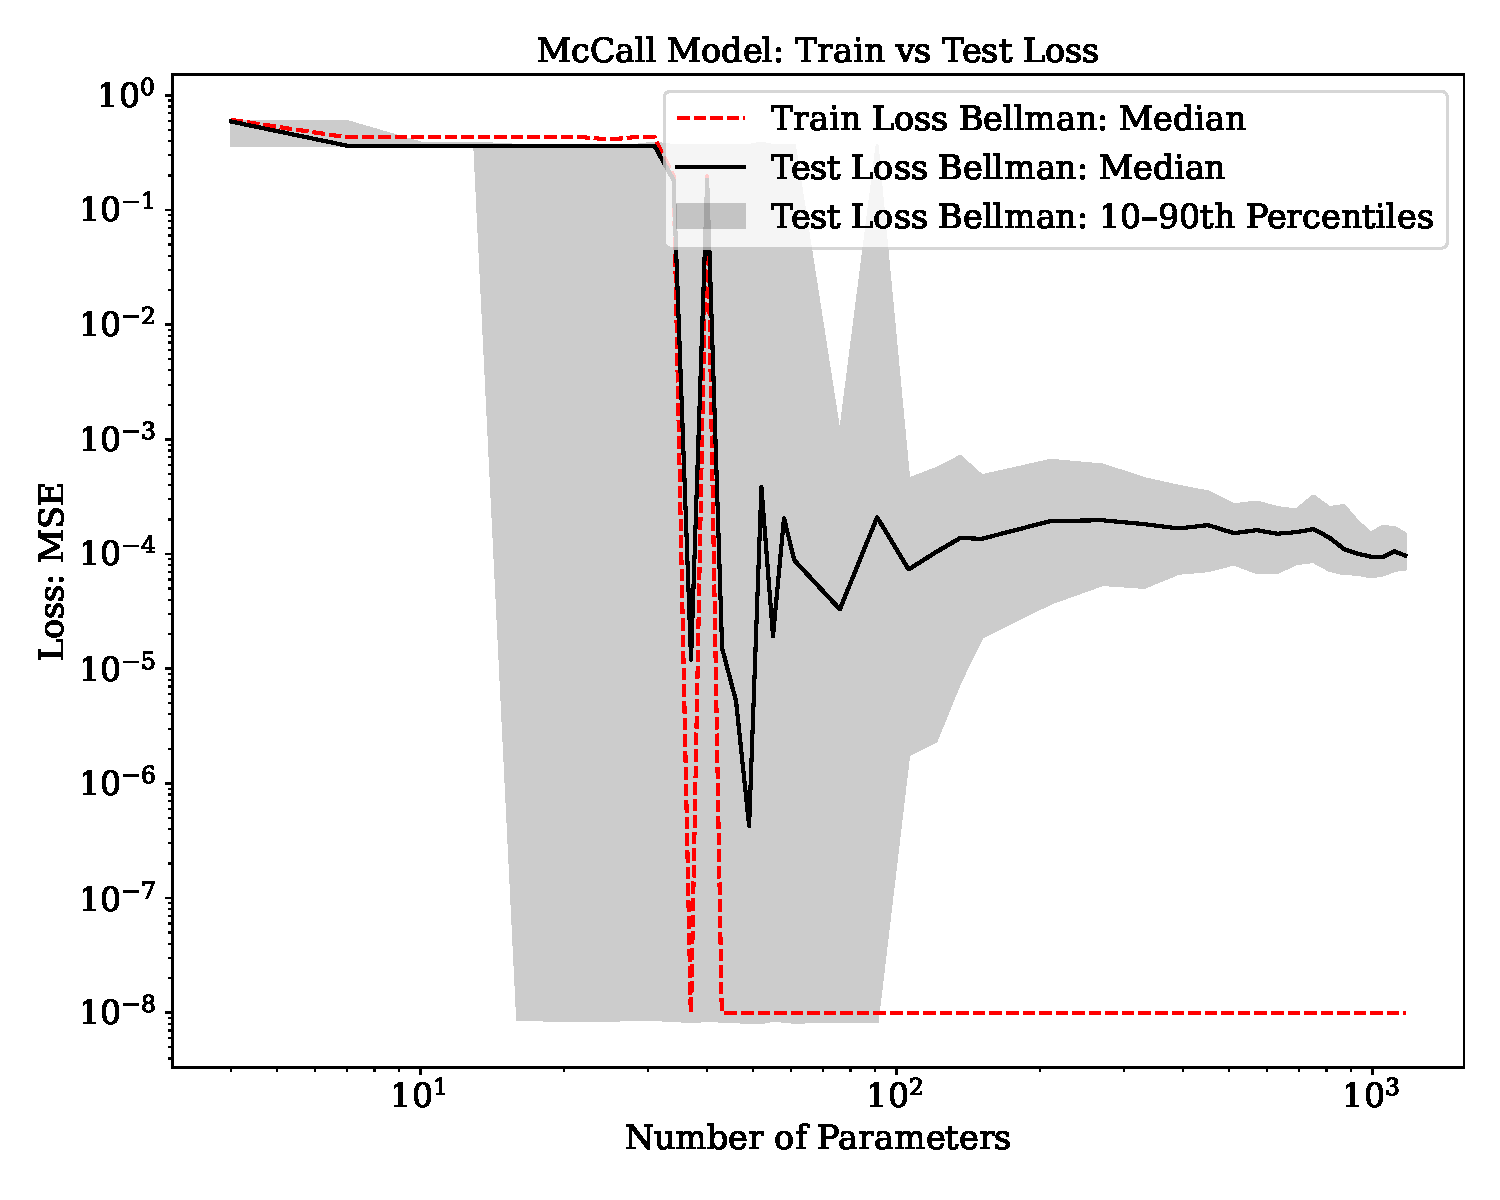
\includegraphics[width=\textwidth]{figures/Mccall_test_train_loss.pdf}
		\end{column}
		\begin{column}{0.45\textwidth}
			\begin{itemize}
				\item Test loss descends again in the overparameterized regime: the \emphcolor{double-descent pattern}?.
				\item The across-seed band collapses.
			\end{itemize}
		\end{column}
	\end{columns}
\end{frame}

\begin{frame}{McCall: absolute relative error}
	\begin{figure}[t!]
		\centering
		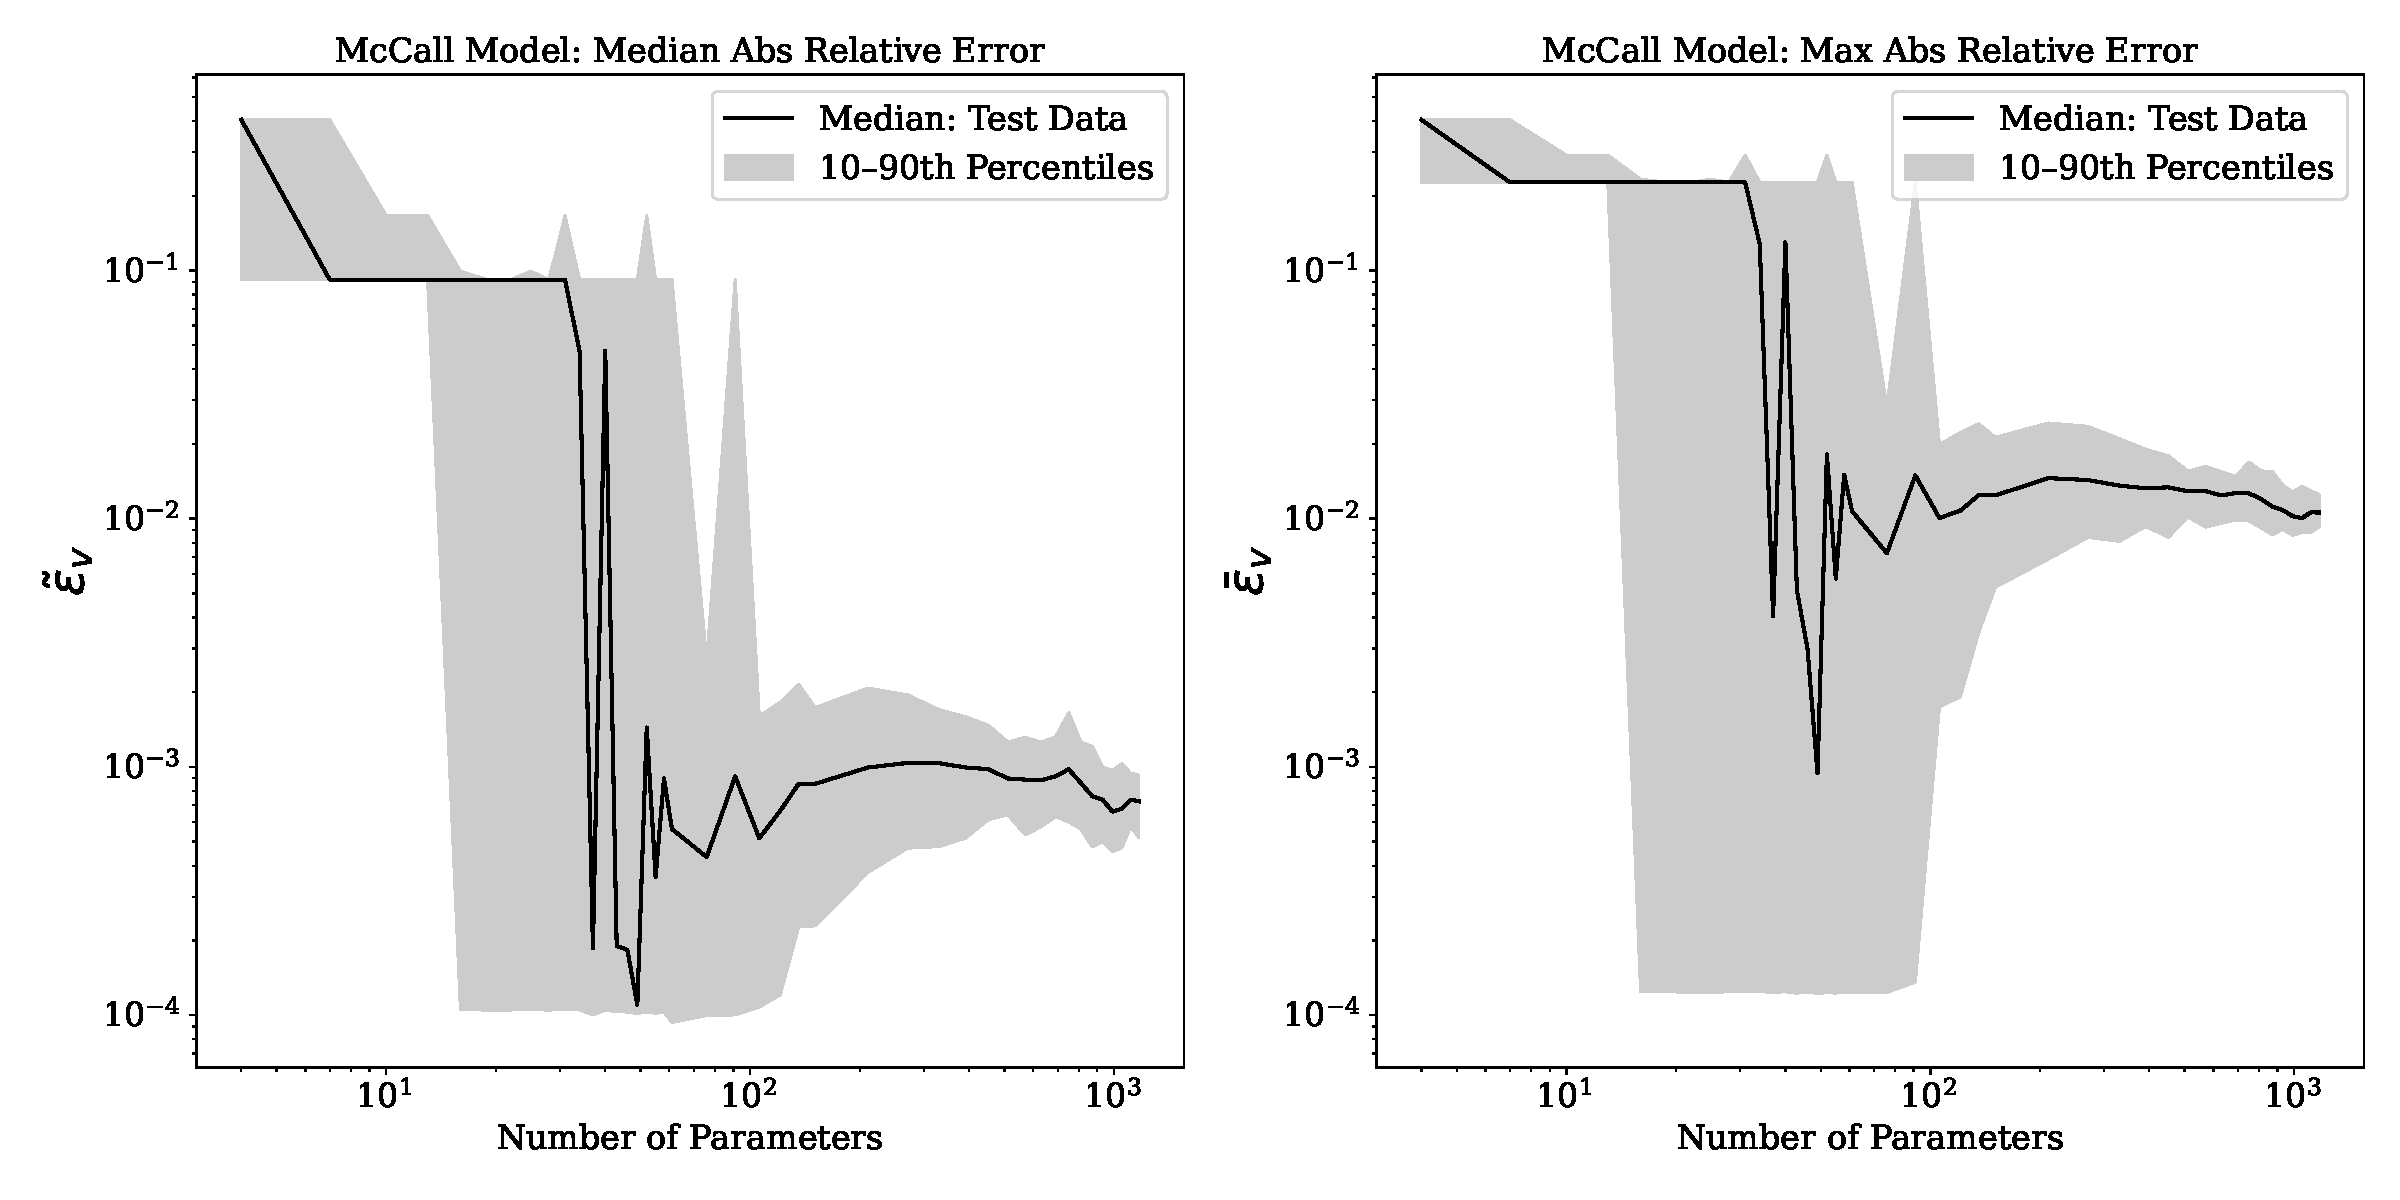
\includegraphics[width=0.8\textwidth]{figures/Mccall_rel_error_median_vs_max.pdf}
	\end{figure}
	\begin{itemize}
		\item Median (left) and max (right) relative error fall from $\sim$30\% to $\sim$2\% as the network enters the overparameterized regime.
		\item The across-seed band narrows sharply: \emphcolor{stability blessing confirmed}.
	\end{itemize}
\end{frame}

\begin{frame}{McCall: value function, underparameterized vs.\ overparameterized}
	\begin{figure}[t!]
		\centering
		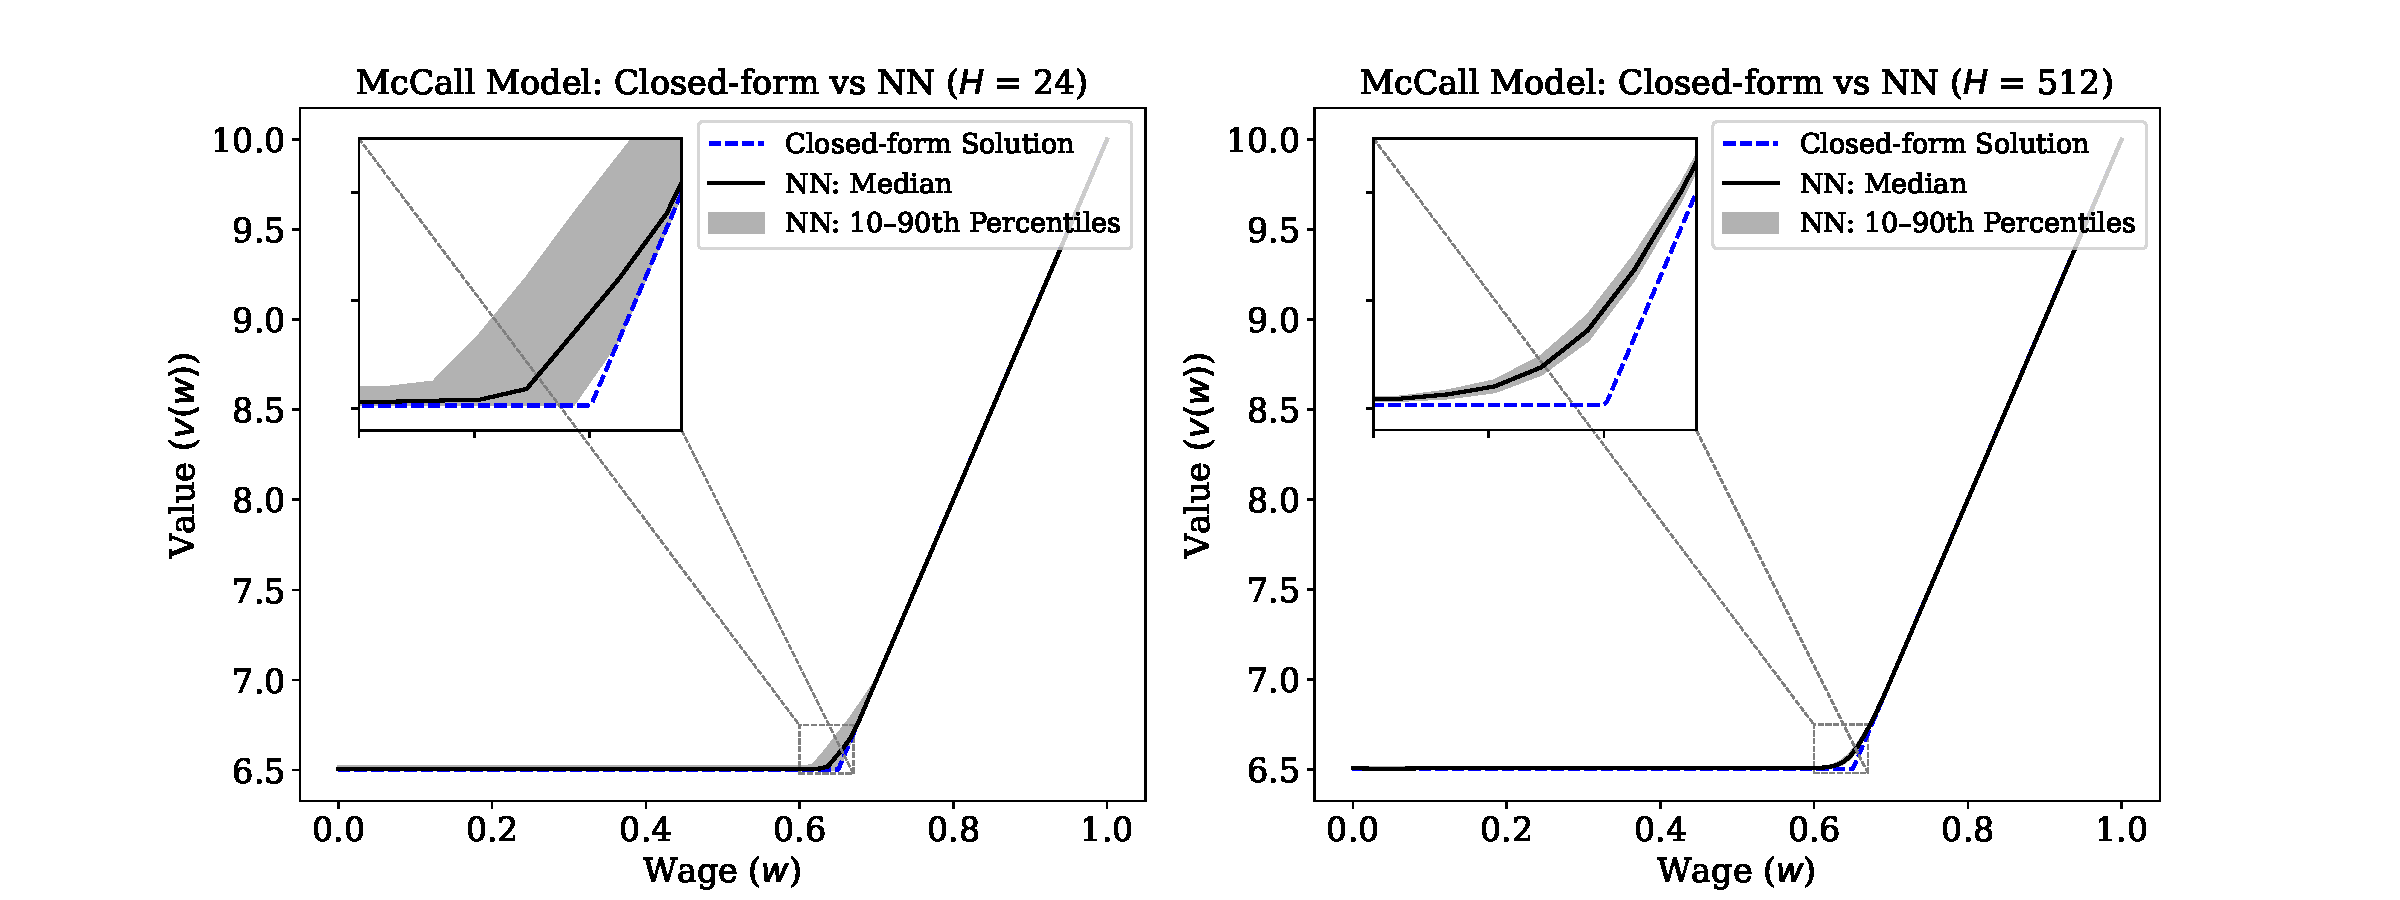
\includegraphics[width=0.85\textwidth]{figures/McCall_value_function_24_vs_512.pdf}
	\end{figure}
	\begin{itemize}
		\item Left: $H = 24$ (underparameterized). Median tracks the closed-form solution well, but the across-seed band is wide.
		\item Right: $H = 512$ (overparameterized). Band is nearly invisible: 50 random initializations converge to the same function.
	\end{itemize}
\end{frame}

%=====================================================================
\section{\textcolor{KahouBlack}{Application 3: Real Business Cycle model}}
%=====================================================================

\begin{frame}{From deterministic to stochastic, from closed form to none}
	\begin{itemize}
		\item The LQ model is linear with a closed-form solution. The McCall model is nonlinear with a kink but still one-dimensional and still admits a closed form.
		\item The Real Business Cycle model (\textcolor{emphcolorval}{Kydland and Prescott, 1982}) is the most demanding test: a two-dimensional stochastic state space $(k_t, z_t)$ and no analytical solution.
		\item Social planner, Cobb--Douglas production $e^{z_t} k_t^\alpha$, stochastic TFP:
		\begin{empheq}[box=\tcbhighmath]{align*}
			&\max_{\{c_t, k_{t+1}\}} \mathbb{E}_0 \sum_{t=0}^\infty \beta^t u(c_t) \quad \st\quad c_t + k_{t+1} = e^{z_t} k_t^\alpha + (1-\delta)k_t \\
			&z_t = \rho z_{t-1} + \sigma \varepsilon_t, \qquad \varepsilon_t \sim \mathcal{N}(0,1)
		\end{empheq}
		\item Key object: policy function $k'(k,z)$. Benchmark: value function iteration (VFI) on a fine grid.
	\end{itemize}
\end{frame}

\begin{frame}{RBC: the Euler equation}
	\begin{itemize}
		\item Euler equation:
		\begin{empheq}[box=\tcbhighmath]{align*}
			u'(c_t) = \beta\, \mathbb{E}_t\!\left[ u'(c_{t+1}) \left( \alpha e^{z_{t+1}} k_{t+1}^{\alpha-1} + 1 - \delta \right) \right]
		\end{empheq}
		\item \emphcolor{LHS}: marginal utility cost of saving one unit today.
		\item \emphcolor{RHS}: expected discounted marginal utility gain from extra capital tomorrow (marginal product plus undepreciated capital).
		\item Nonlinearity plus stochastic two-dimensional state means no analytical solution.
		\item This is the operator equation from slide 1, now in its full stochastic form.
	\end{itemize}
\end{frame}

\begin{frame}{Parameterization}
	\vspace{0.2in}
	\begin{center}
		\begin{tabular}{llcl}
			\toprule
			Description & Symbol & Value & \\
			\midrule
			Discount factor   & $\beta$  & \textcolor{emphcolorval}{0.96} & \\
			Capital share     & $\alpha$ & \textcolor{emphcolorval}{1/3}  & Cobb--Douglas exponent \\
			Depreciation rate & $\delta$ & \textcolor{emphcolorval}{0.1}  & per-period capital depreciation \\
			TFP persistence   & $\rho$   & \textcolor{emphcolorval}{0.9}  & AR(1) coefficient for $z_t$ \\
			TFP volatility    & $\sigma$ & \textcolor{emphcolorval}{0.01} & std.\ dev.\ of $\varepsilon_t$ \\
			Utility function  & $u(c)$   & \textcolor{emphcolorval}{$\ln c$} & log utility \\
			\bottomrule
		\end{tabular}
	\end{center}
\end{frame}

\begin{frame}{RBC: deep learning implementation}
	\begin{itemize}
		\item \emphcolor{Architecture:} one-hidden-layer ReLU network $k'(k,z;\theta)$. Output layer: Softplus activation $\log(1+e^x)$ to enforce $k' > 0$. 50 seeds per width.
		\item \emphcolor{Training:} $20 \times 20$ Cartesian grid ($N = 400$). Euler residual:
		\begin{empheq}[box=\tcbhighmath]{align*}
			\ell_{\mathrm{Euler}}(k,z;\theta) = \frac{1}{c(k,z;\theta)} - \beta \sum_{i=1}^M \frac{w_i}{\sqrt{\pi}} \left[ \frac{\alpha e^{\rho z + \sqrt{2}\sigma \zeta_i} k'(k,z;\theta)^{\alpha-1} + 1 - \delta}{c\big(k'(k,z;\theta),\, \rho z + \sqrt{2}\sigma \zeta_i;\, \theta\big)} \right]
		\end{empheq}
		with $M = 15$ Gauss--Hermite nodes. Adam with StepLR scheduler.
		\item \emphcolor{Penalty term:} $\lambda\big(k'(k^*,0;\theta) - k^*\big)^2$ with $\lambda = 0.01$, enforcing a necessary implication of the transversality condition at the steady state.
	\end{itemize}
\end{frame}

\begin{frame}{RBC: why the penalty term?}
	\begin{itemize}
		\item The Euler equation is a \emph{necessary but not sufficient} condition for optimality.
		\item Both the stable and explosive solution manifolds through the steady state satisfy it identically.
		\item What rules out explosive solutions is the transversality condition (TVC):
		\begin{align*}
			\lim_{t\to\infty} \beta^t u'(c_t) k_{t+1} = 0
		\end{align*}
		\item The Euler residual loss does not enforce the TVC directly.
		\item The penalty resolves this multiplicity by imposing $k'(k^*,0) = k^*$: the steady state is a fixed point of the policy function.
		\item Without this, gradient-based training can converge to the explosive manifold: small Euler residuals but divergent simulated paths.
	\end{itemize}
\end{frame}

\begin{frame}{RBC: training and test data}
	\begin{columns}
		\begin{column}{0.55\textwidth}
			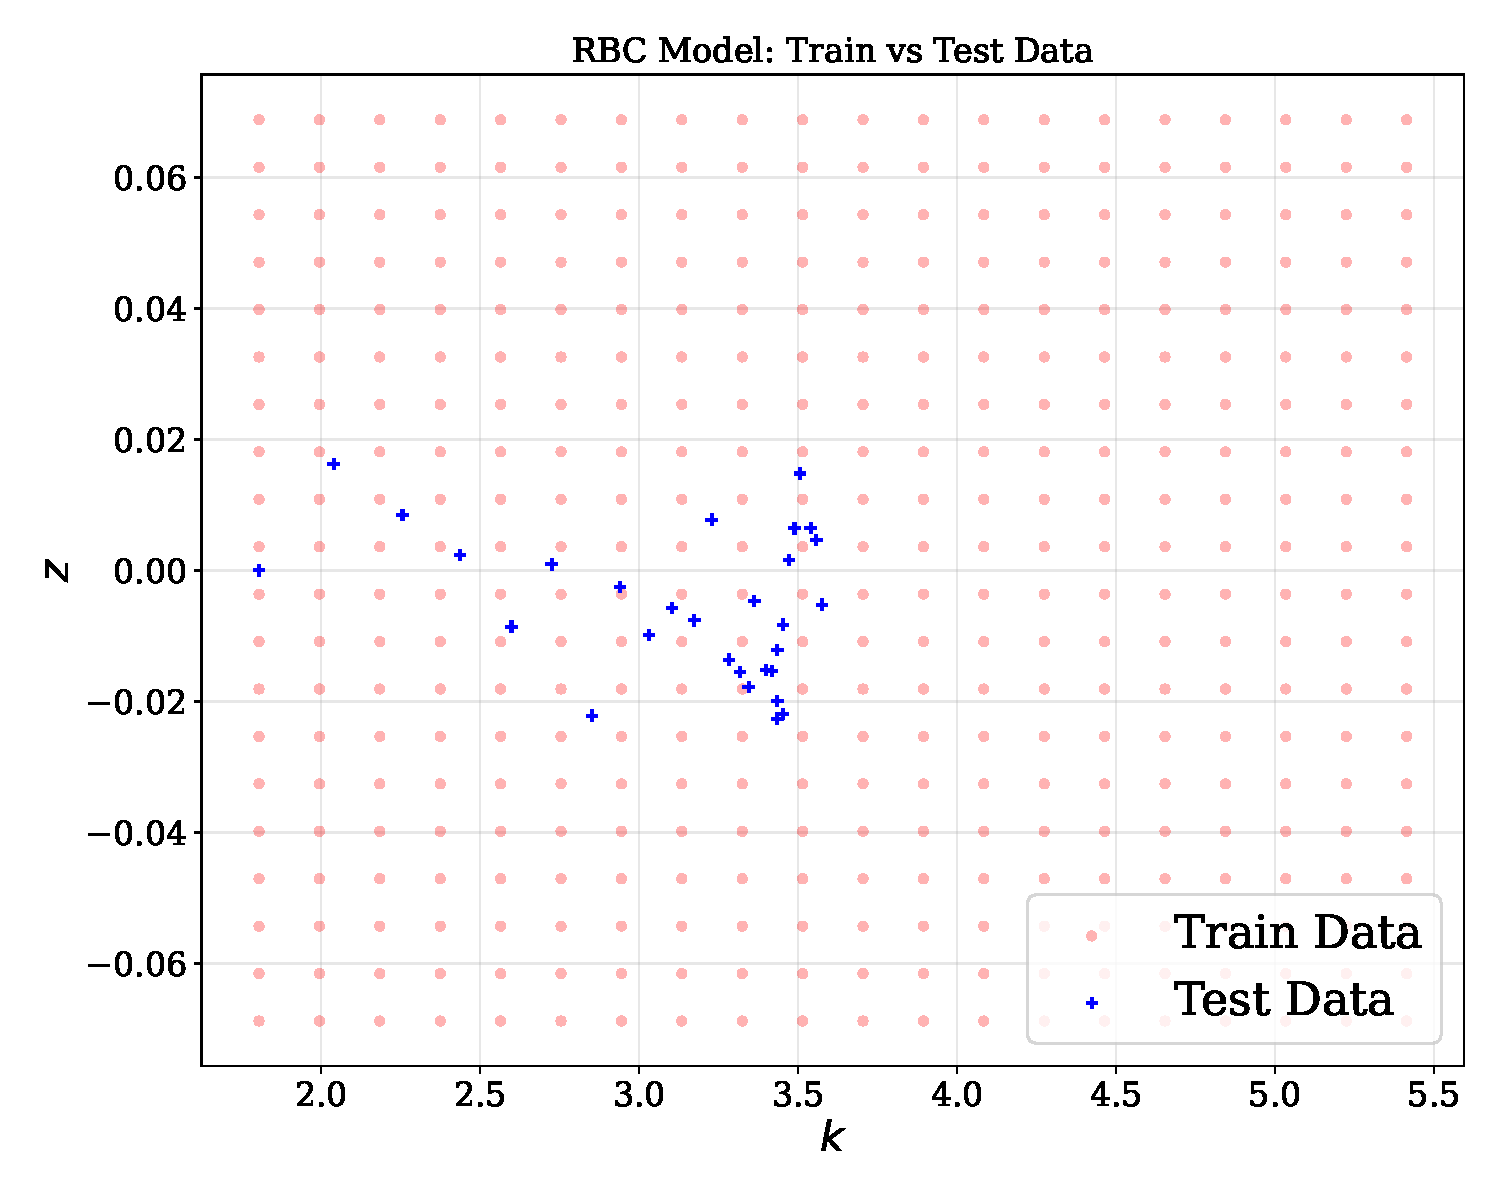
\includegraphics[width=\textwidth]{figures/RBC_test_vs_train_data.pdf}
		\end{column}
		\begin{column}{0.45\textwidth}
			\begin{itemize}
				\item Red dots: \textcolor{emphcolorval}{$20 \times 20$} training grid.
				\item Blue crosses: \textcolor{emphcolorval}{$T = 29$} path simulated under the VFI policy starting at $k_0 = 0.5\, k^*$.
				\item Test path visits the interior of the state space and is never on a training node.
			\end{itemize}
		\end{column}
	\end{columns}
\end{frame}

\begin{frame}{RBC: train and test Euler-residual loss}
	\begin{columns}
		\begin{column}{0.55\textwidth}
			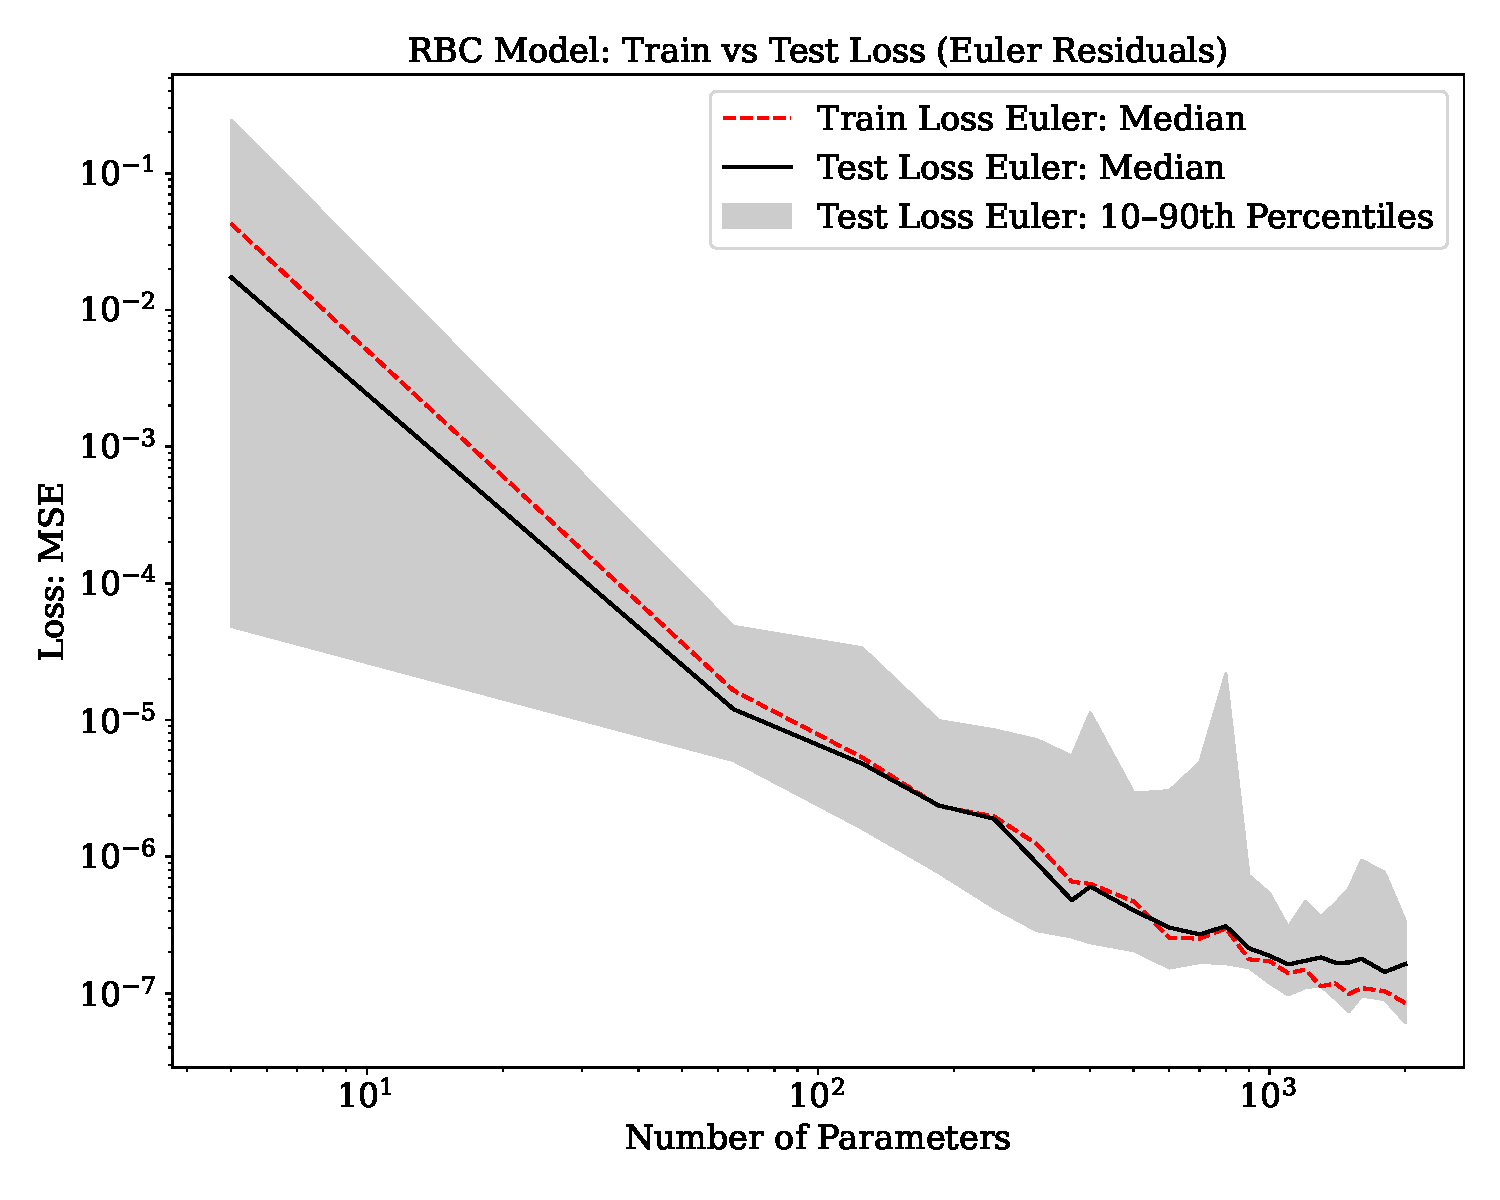
\includegraphics[width=\textwidth]{figures/RBC_test_train_loss.pdf}
		\end{column}
		\begin{column}{0.45\textwidth}
			\begin{itemize}
				\item Both losses decline as the network grows wider, with no \emphcolor{sign of overfitting}.
				\item The across-seed band narrows sharply: overparameterization simultaneously improves accuracy and reduces initialization sensitivity.
			\end{itemize}
		\end{column}
	\end{columns}
\end{frame}

\begin{frame}{RBC: absolute relative error vs.\ VFI}
	\begin{figure}[t!]
		\centering
		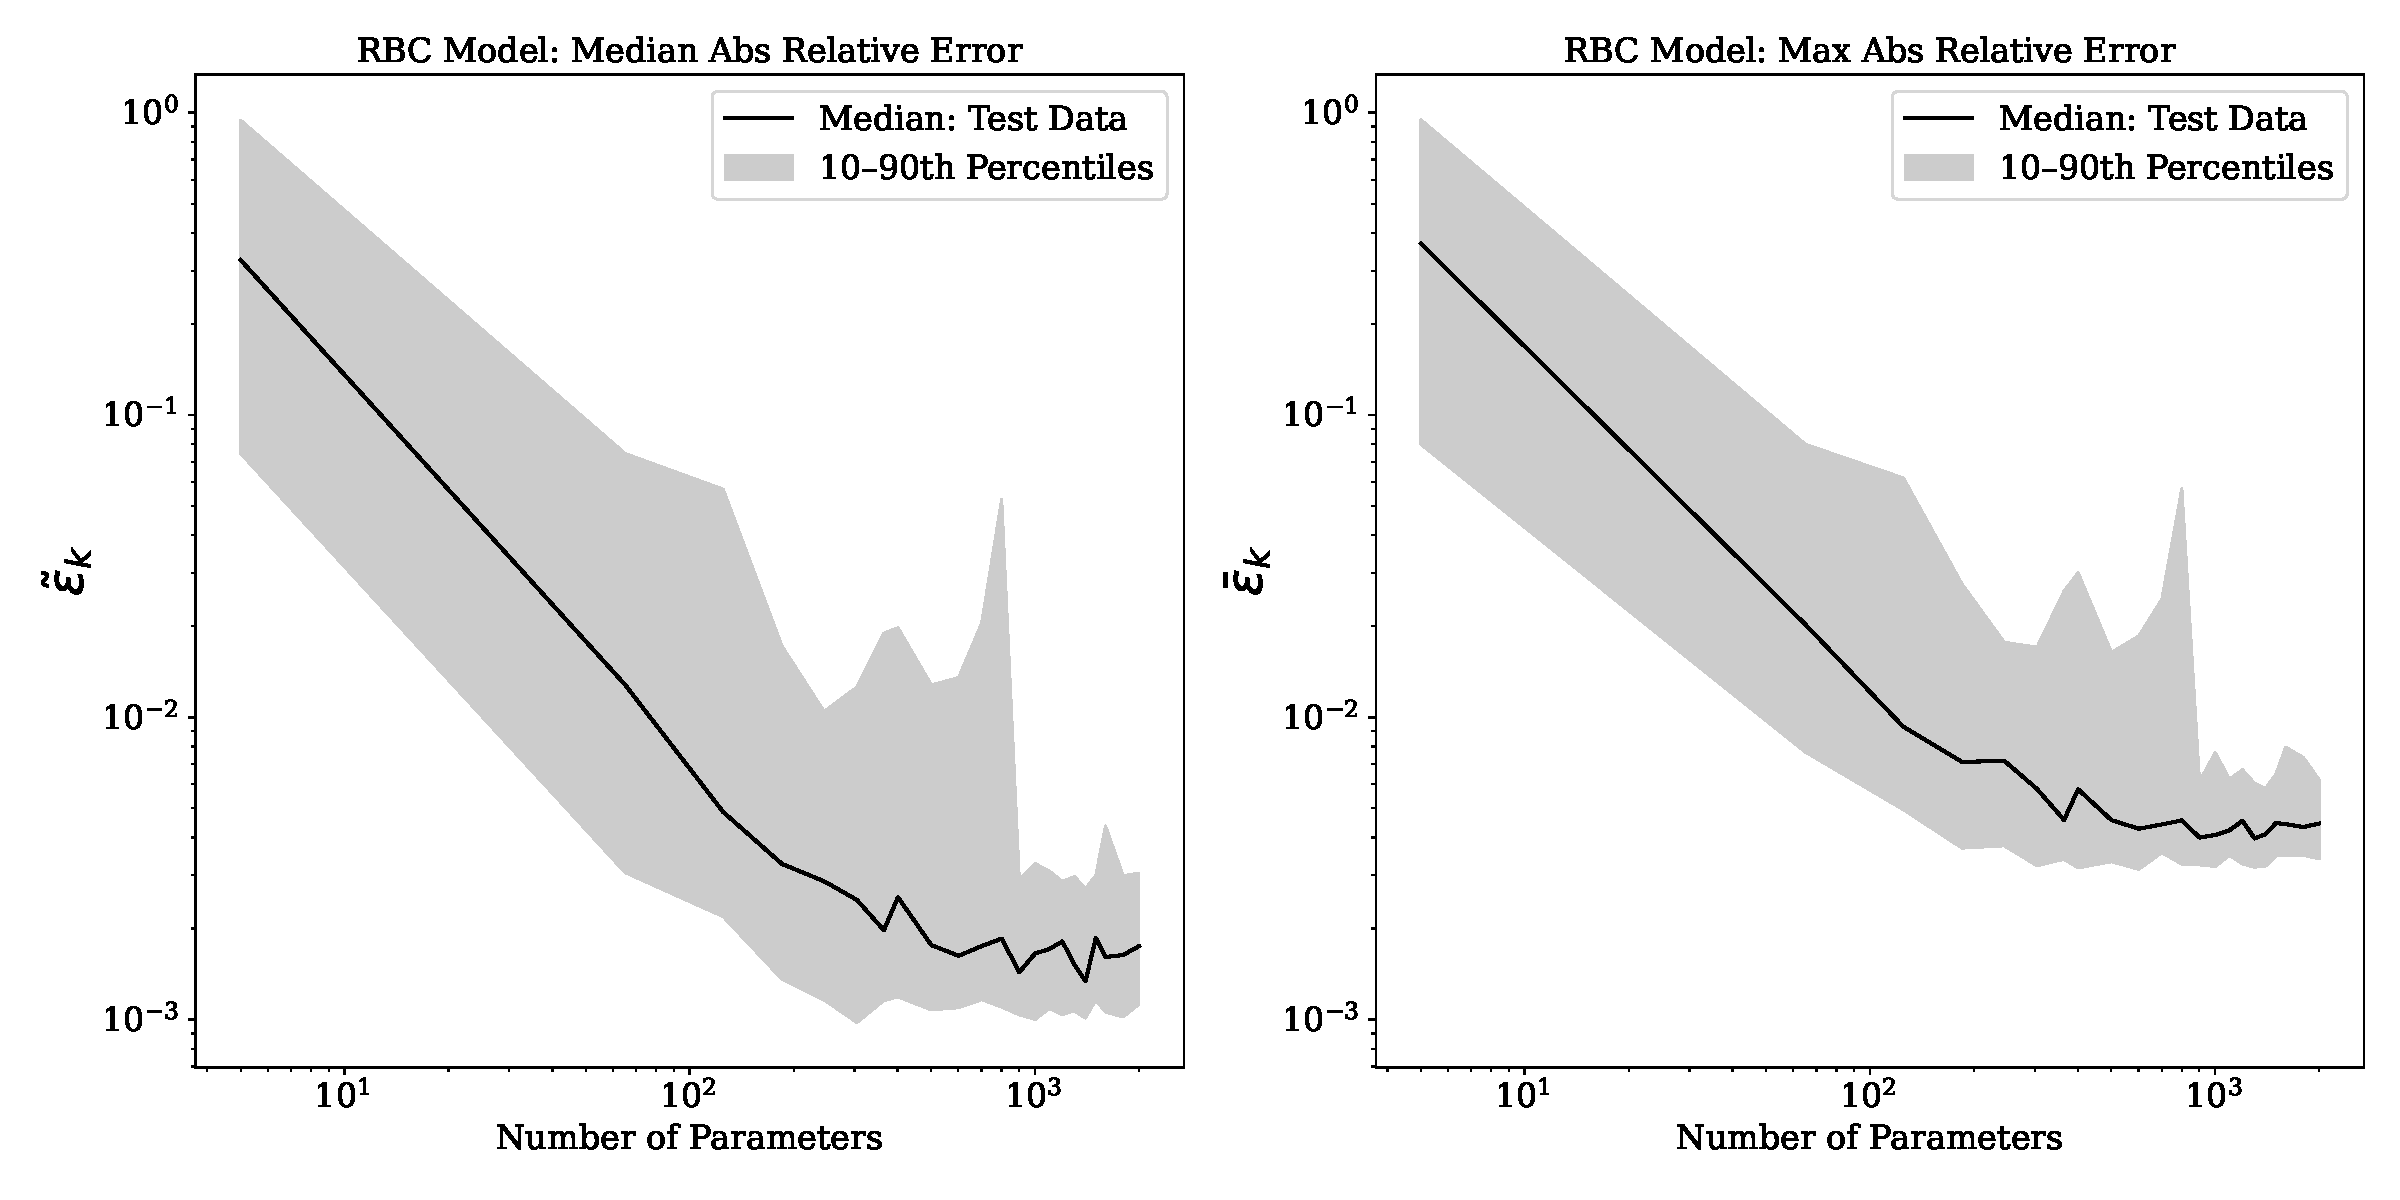
\includegraphics[width=0.85\textwidth]{figures/RBC_rel_error_median_vs_max.pdf}
	\end{figure}
	\begin{itemize}
		\item Median (left) and maximum (right) absolute relative error of the NN capital policy versus VFI.
		\item Both statistics decline and concentrate around the median seed as width increases.
	\end{itemize}
\end{frame}

\begin{frame}{RBC: capital paths, underparameterized vs.\ overparameterized}
	\begin{figure}[t!]
		\centering
		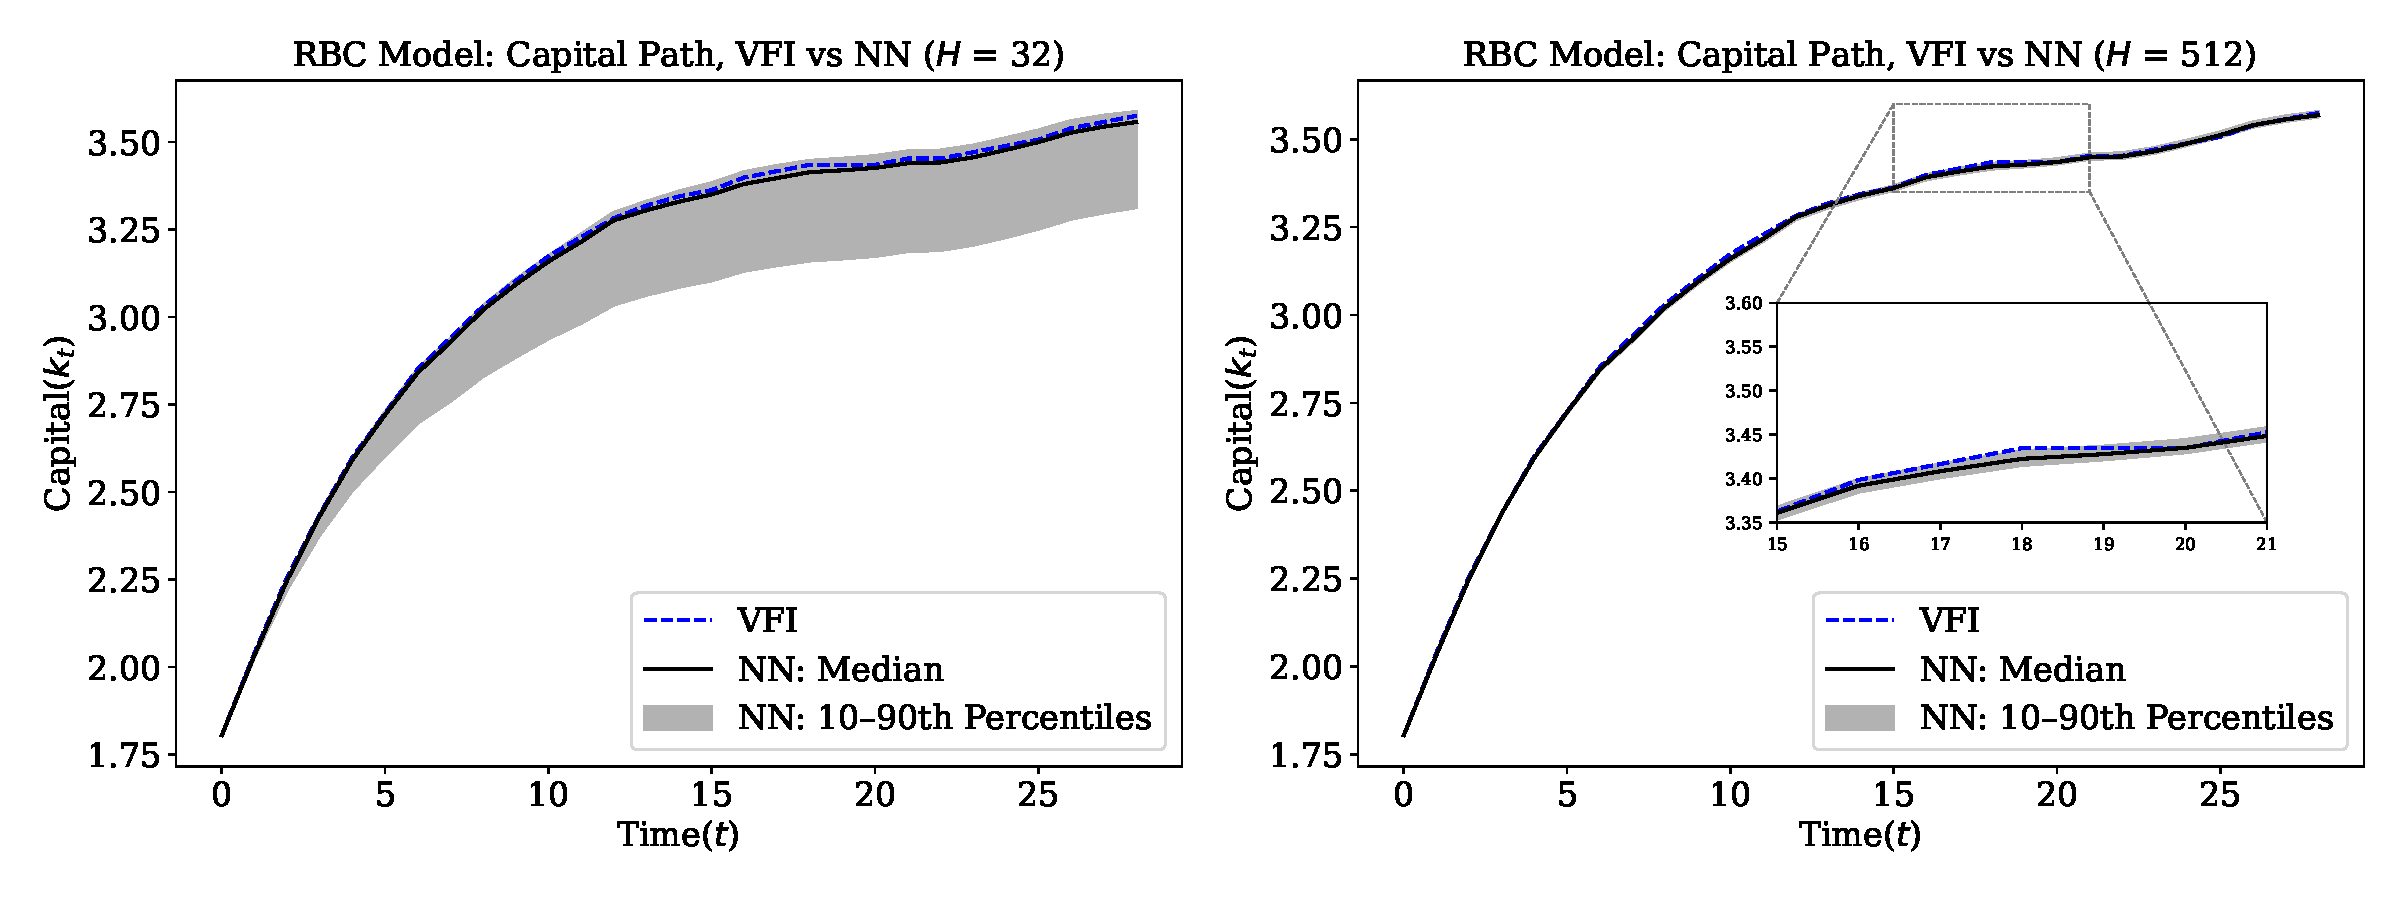
\includegraphics[width=0.85\textwidth]{figures/RBC_capital_path_32_vs_512.pdf}
	\end{figure}
	\begin{itemize}
		\item Left: $H = 32$. Median path close to VFI, but across-seed band is wide. Accurate on average but unreliable.
		\item Right: $H = 512$. Median tracks VFI almost exactly over the full horizon \emph{and} the band collapses to near zero.
	\end{itemize}
\end{frame}

%=====================================================================
\section{\textcolor{KahouBlack}{Robustness}}
%=====================================================================

\begin{frame}{Are these results specific to ReLU and one hidden layer?}
	\vspace{0.1in}
	\begin{itemize}
		\item A natural concern: the blessing might depend on the particular activation function or the single-layer architecture.
		\item We test robustness along two dimensions:
		\begin{itemize}
			\item \emphcolor{Activation functions:} Sigmoid and Leaky ReLU in addition to the baseline ReLU.
			\item \emphcolor{Network depth:} two-hidden-layer architectures in addition to the baseline one-hidden-layer.
		\end{itemize}
	\end{itemize}
	\begin{block}{Result}
		The blessing holds in every configuration we tried. The next slides document this for each model.
	\end{block}
\end{frame}

\begin{frame}{Robustness: alternative activations for the LQ model}
	\begin{columns}
		\begin{column}{0.6\textwidth}
			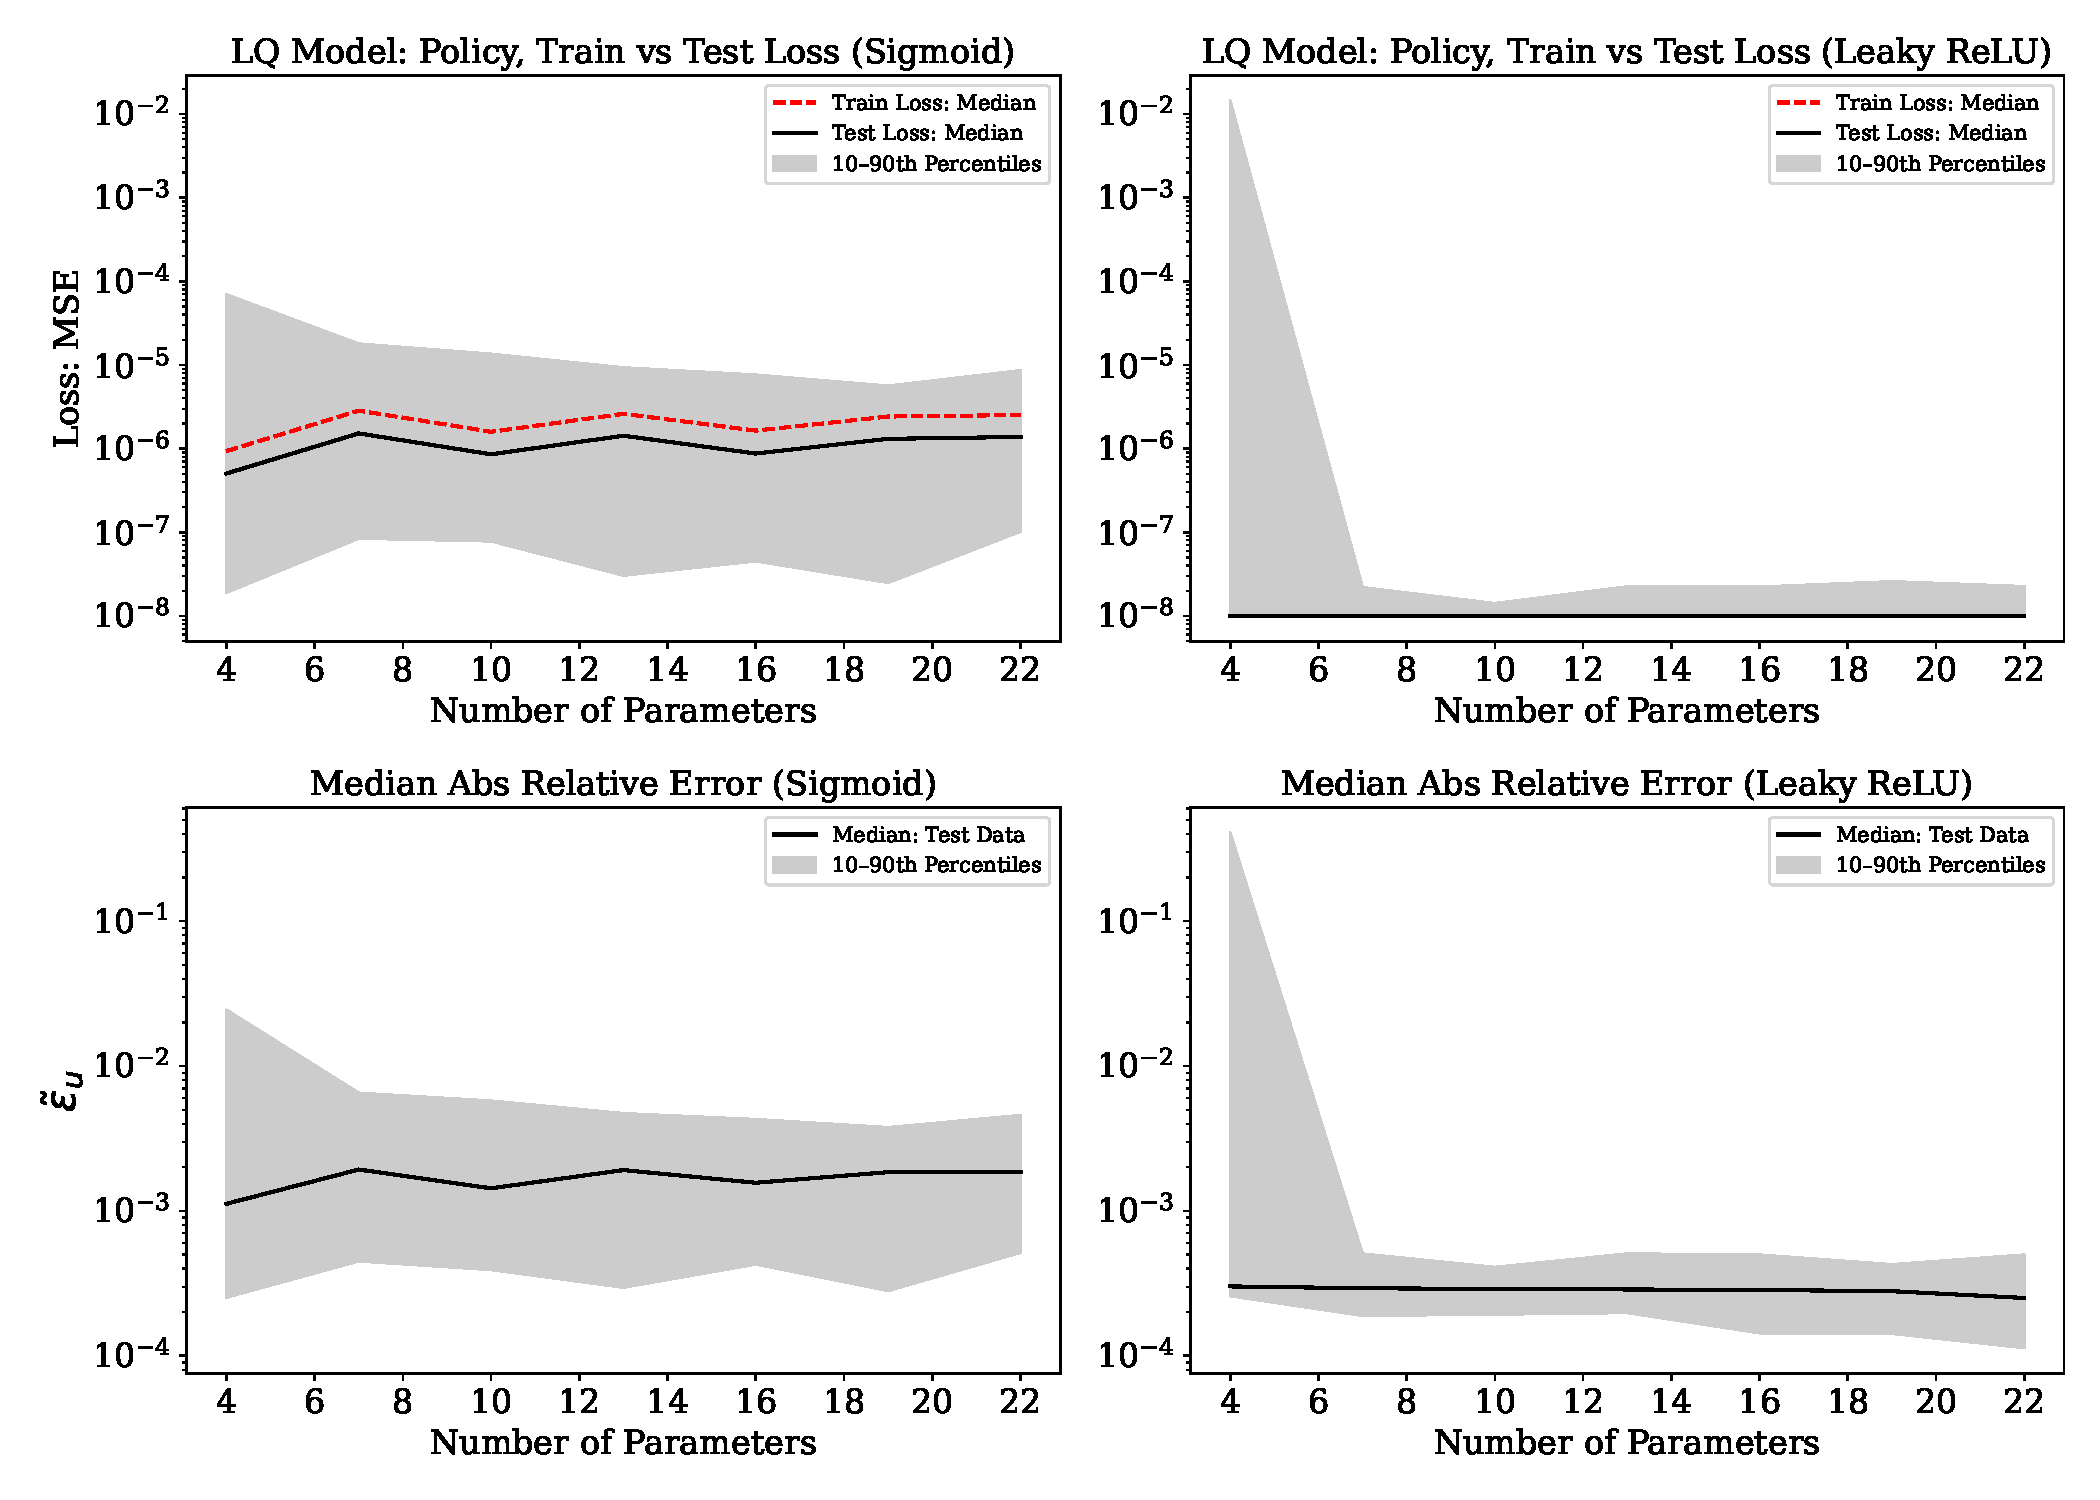
\includegraphics[width=\textwidth]{figures/LQ_policy_robustness_activations.pdf}
		\end{column}
		\begin{column}{0.4\textwidth}
			\begin{itemize}
				\item Sigmoid (left) and Leaky ReLU (right).
				\item Top row: train/test Euler MSE. Bottom row: median relative error.
				\item Both activations replicate the main finding: accuracy improves with width, across-seed dispersion collapses.
			\end{itemize}
		\end{column}
	\end{columns}
\end{frame}

\begin{frame}{Robustness: deeper networks for the McCall model}
	\begin{columns}
		\begin{column}{0.6\textwidth}
			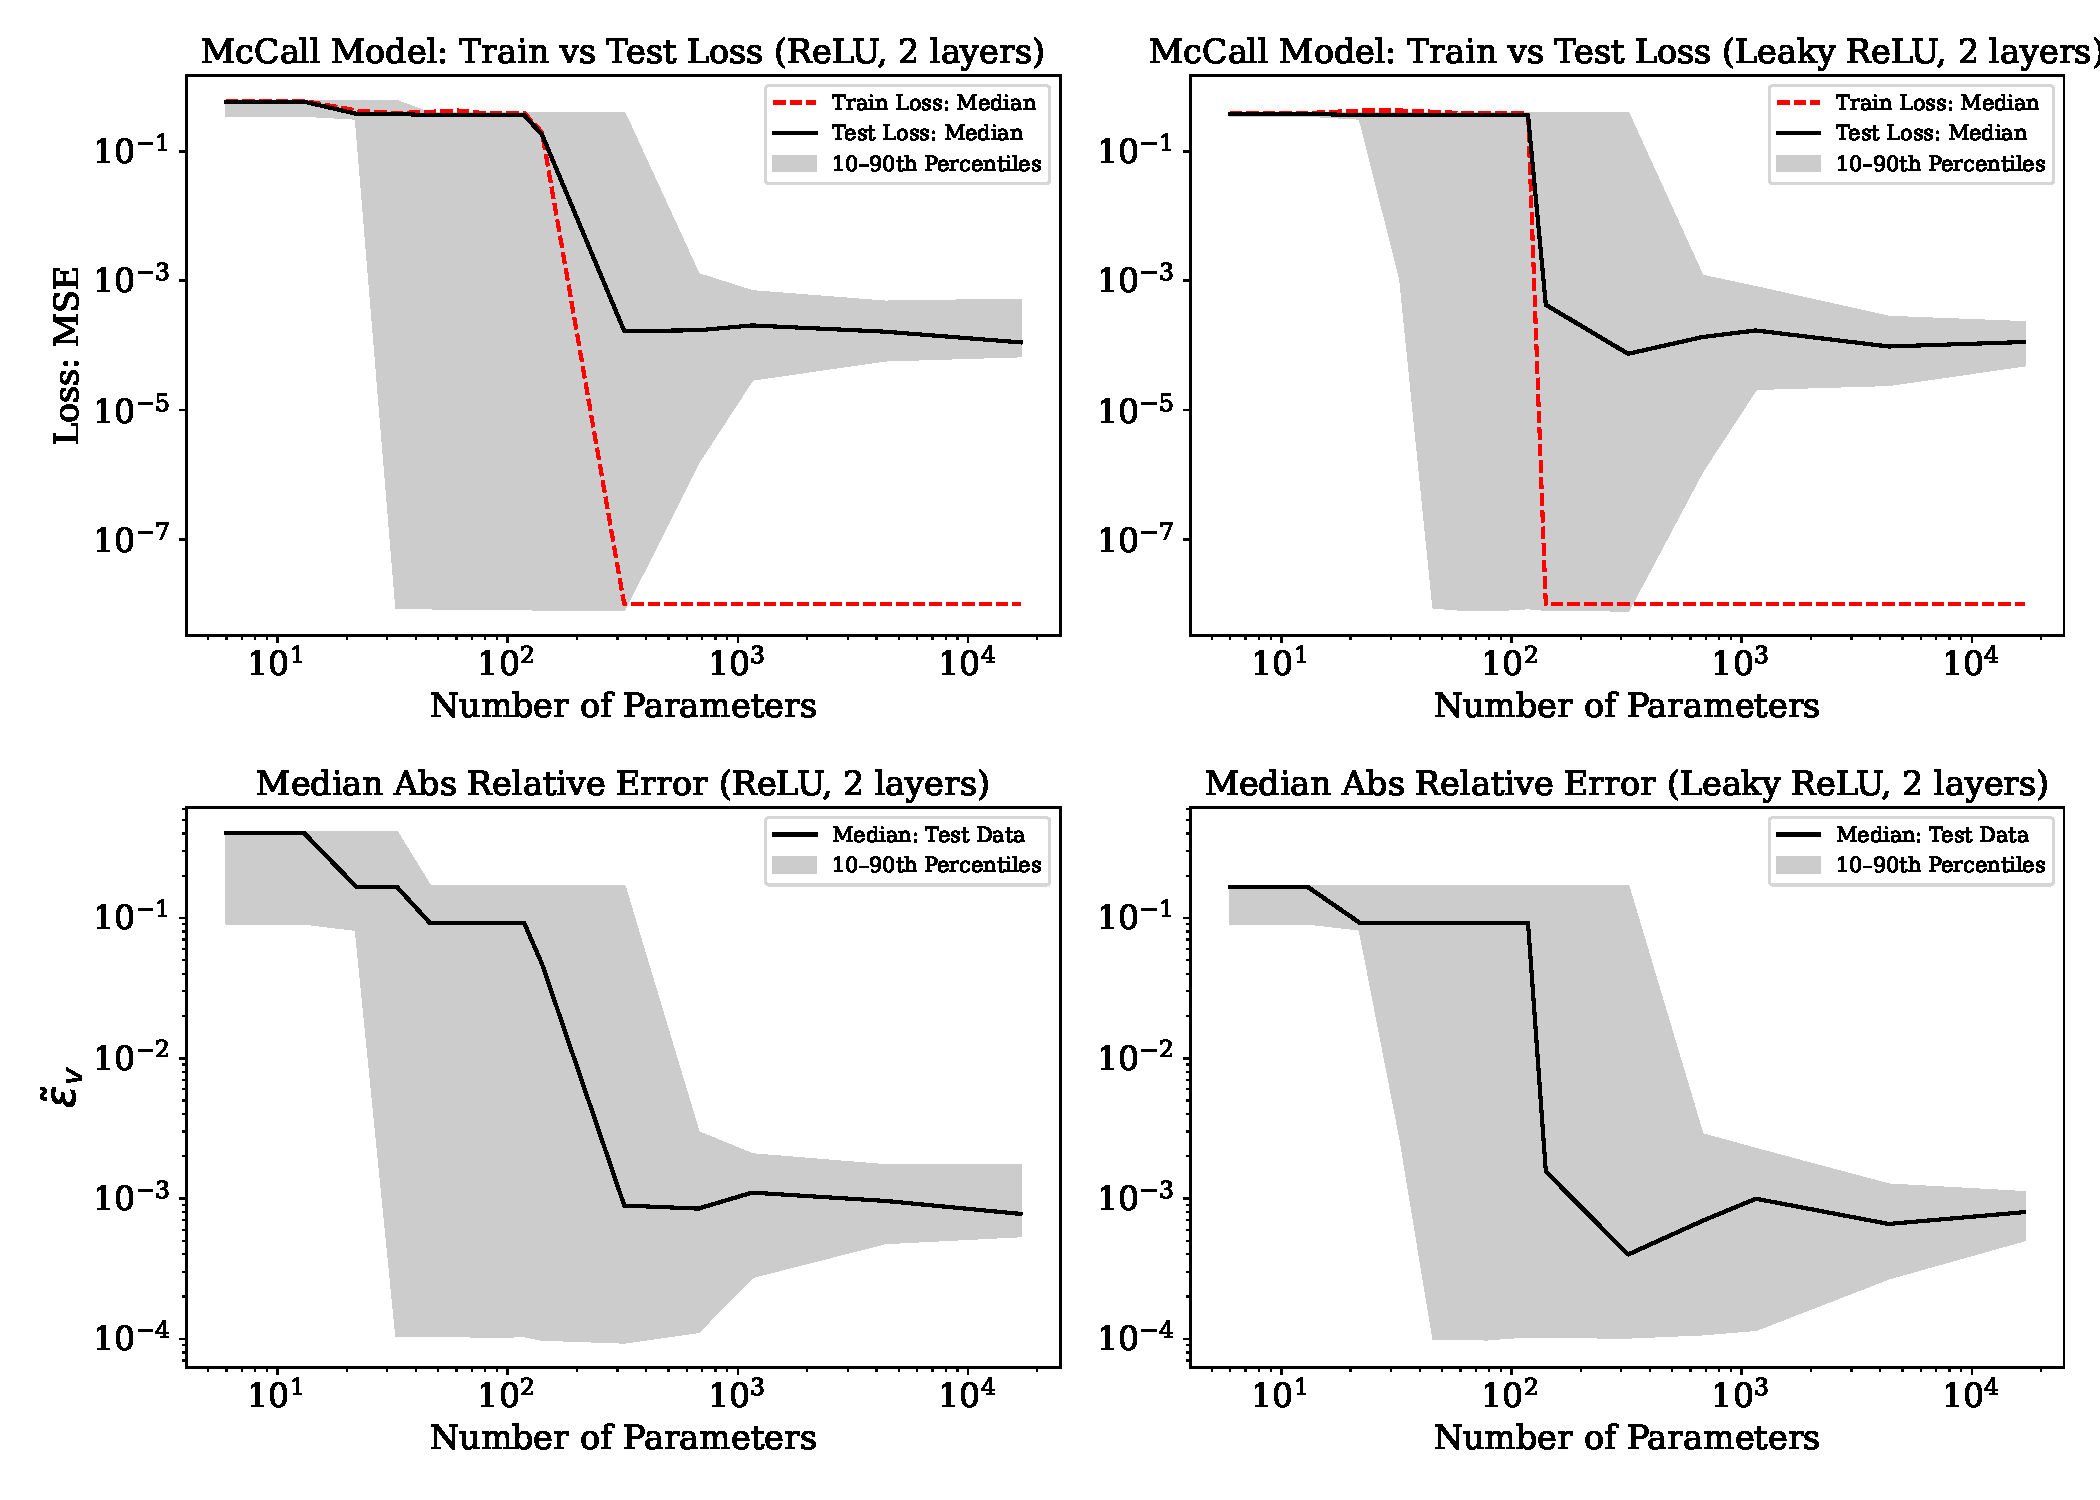
\includegraphics[width=\textwidth]{figures/McCall_robustness_2_layers_activations.pdf}
		\end{column}
		\begin{column}{0.4\textwidth}
			\begin{itemize}
				\item Two-hidden-layer architecture with ReLU (left) and Leaky ReLU (right).
				\item Quantitatively similar results: the blessing is not specific to one-hidden-layer networks.
			\end{itemize}
		\end{column}
	\end{columns}
\end{frame}

\begin{frame}{Robustness: deeper networks for the RBC model}
	\begin{columns}
		\begin{column}{0.6\textwidth}
			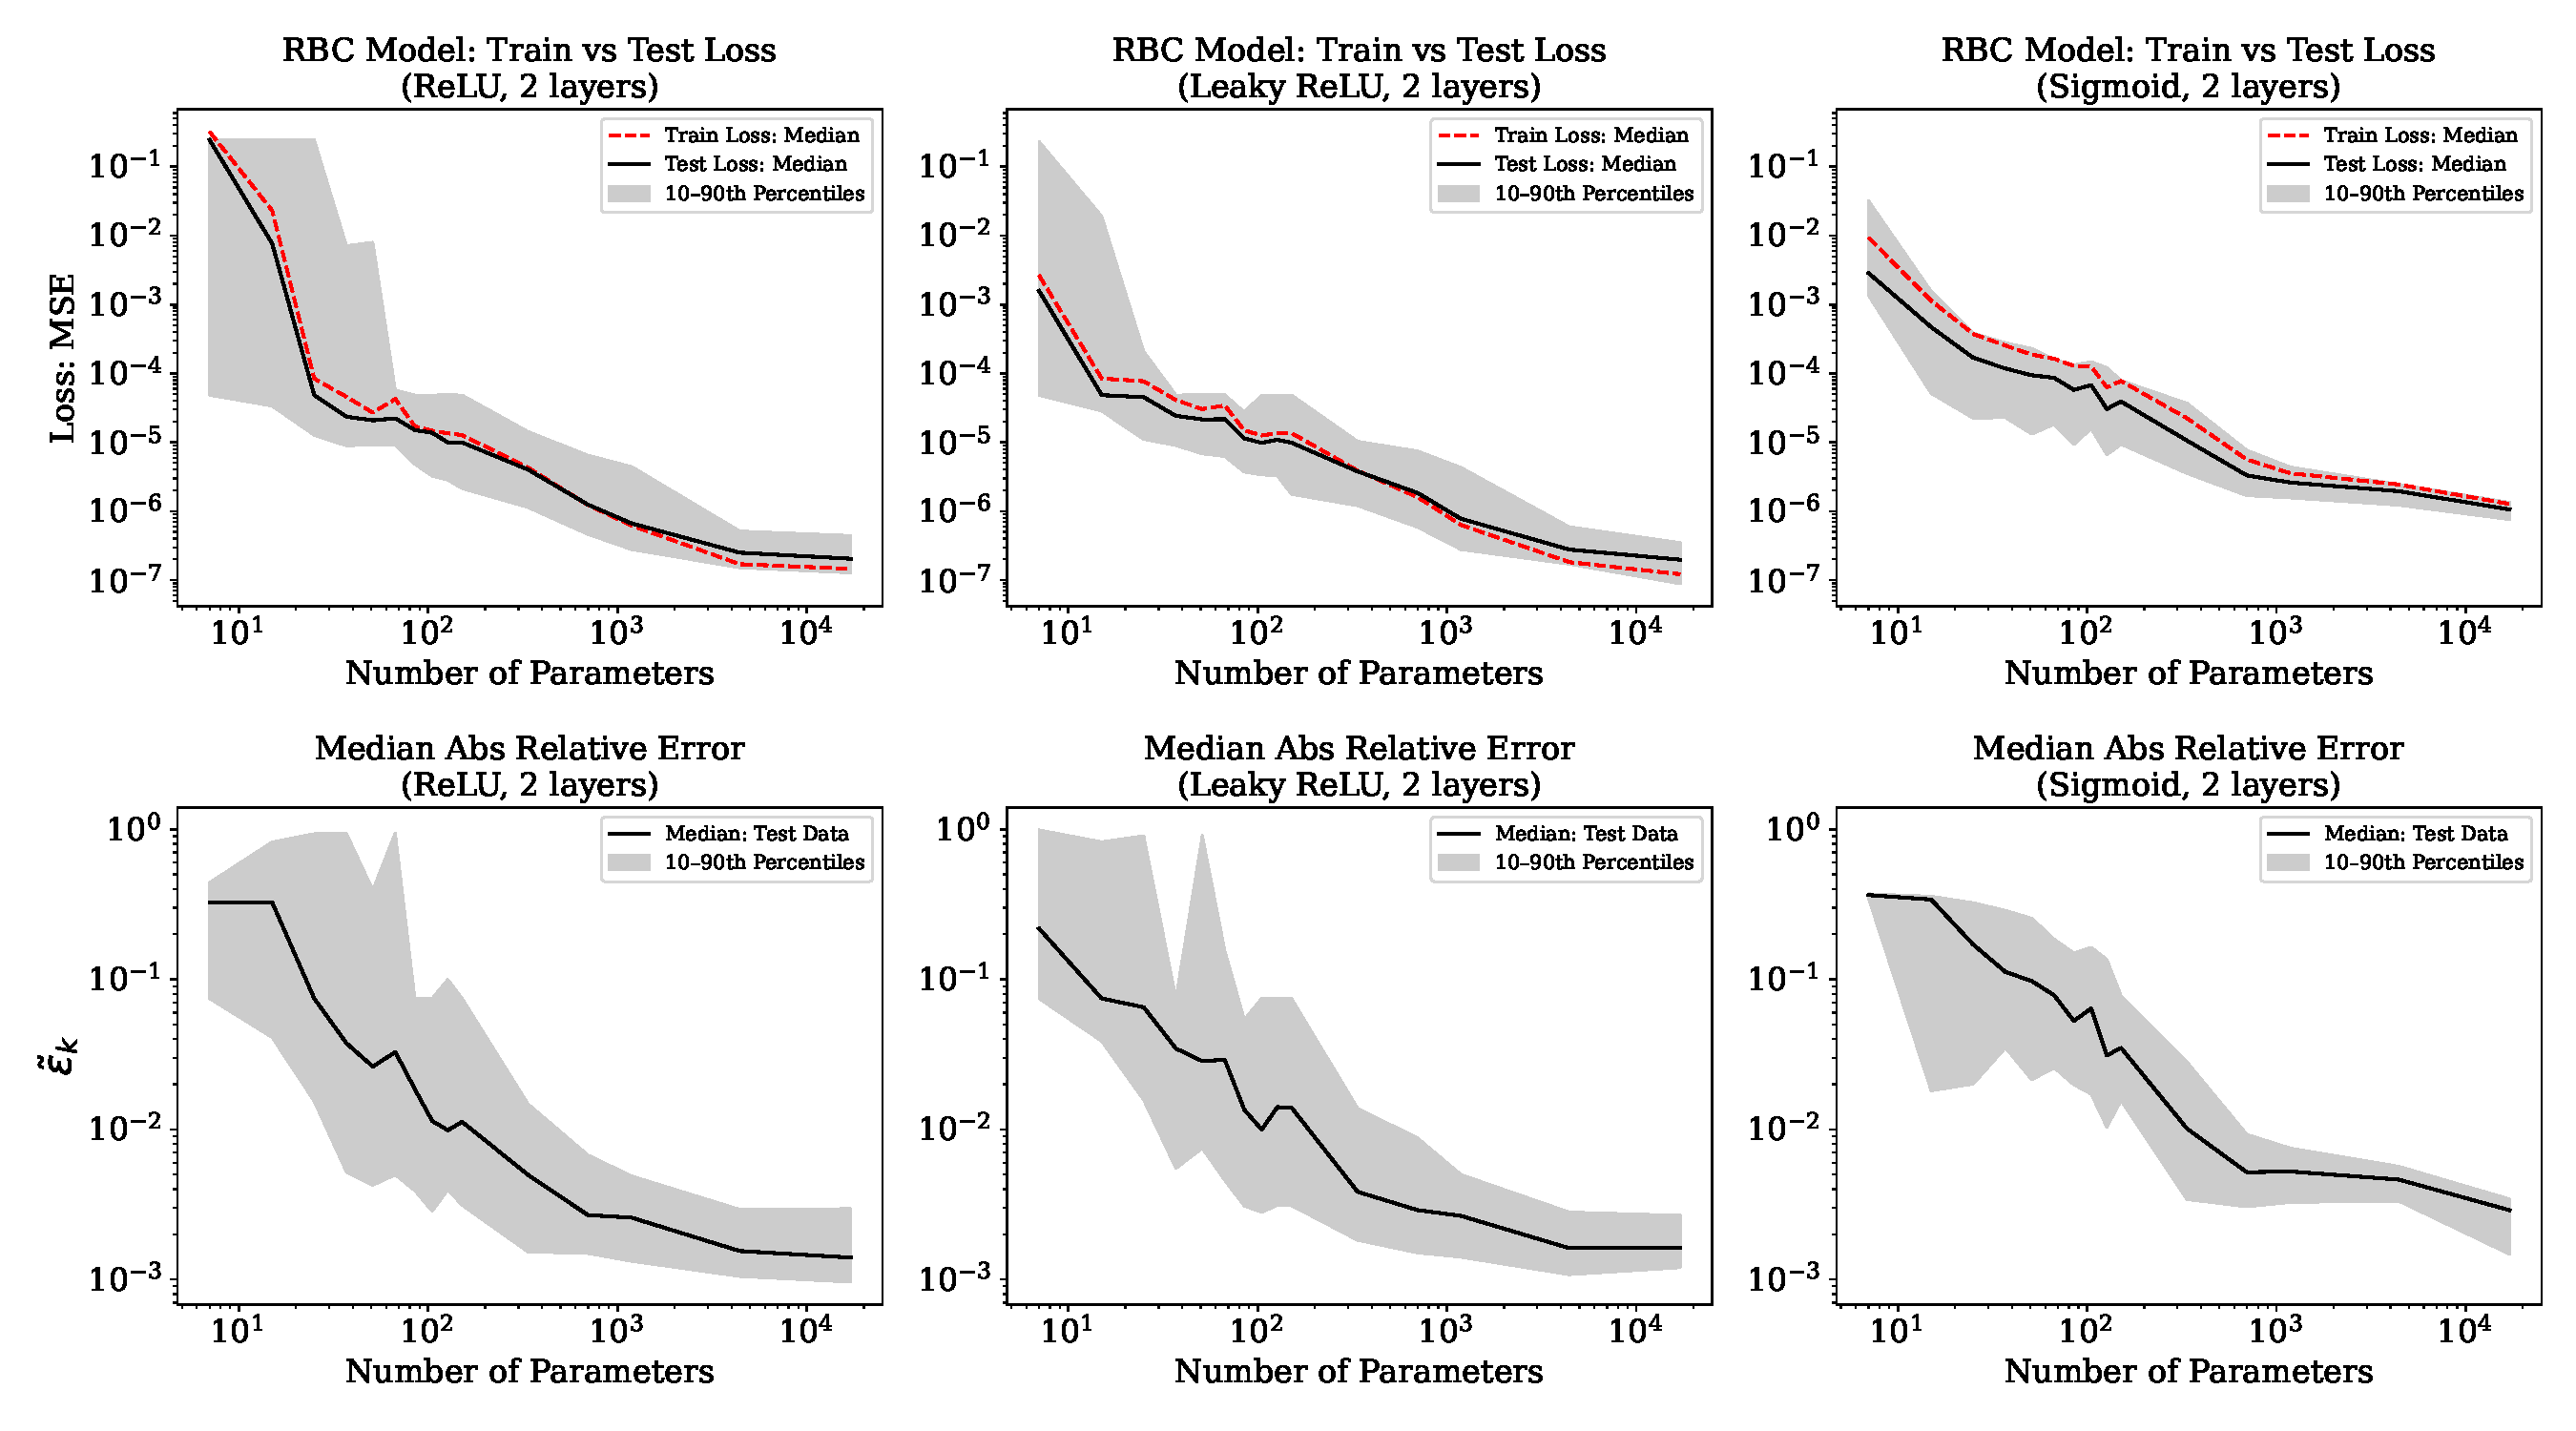
\includegraphics[width=\textwidth]{figures/RBC_robustness_2_layers_activations.pdf}
		\end{column}
		\begin{column}{0.4\textwidth}
			\begin{itemize}
				\item Two-hidden-layer architecture with ReLU (left), Leaky ReLU (center), Sigmoid (right).
				\item All three activations replicate the main finding for a stochastic model with no closed-form solution.
			\end{itemize}
		\end{column}
	\end{columns}
\end{frame}

\begin{frame}{Robustness: summary}
	\vspace{0.1in}
	\begin{itemize}
		\item The blessing of overparameterization is robust across all dimensions most relevant to applied practice:
		\begin{itemize}
			\item \emphcolor{Activation functions:} ReLU, Leaky ReLU, Sigmoid.
			\item \emphcolor{Network depth:} one and two hidden layers.
			\item \emphcolor{Operator type:} Euler residual (LQ, RBC), Bellman residual (McCall).
			\item \emphcolor{Solution regularity:} smooth (LQ), non-smooth with kink (McCall), stochastic without closed form (RBC).
			\item \emphcolor{State dimensionality:} 1D (McCall), 2D (LQ, RBC).
		\end{itemize}
	\end{itemize}
\end{frame}

%=====================================================================
\section{\textcolor{KahouBlack}{Conclusion}}
%=====================================================================

\begin{frame}{Takeaways}
	\begin{itemize}
		\item \emphcolor{Finding 1:} no overfitting. As network width increases, out-of-sample Euler and Bellman residuals decline. Value and policy functions converge toward their benchmarks.
		\item \emphcolor{Finding 2:} algorithmic stability. Small networks produce solutions that depend on the random seed. Wide networks concentrate across seeds, making the algorithm reliable and initialization-independent.
		\item Documented consistently across three operator equations: linear with closed form (LQ), nonlinear with kink (McCall), stochastic with no analytical solution (RBC).
		\item Robust across activations (ReLU, Leaky ReLU, Sigmoid) and depths (one and two hidden layers).
	\end{itemize}
	\begin{block}{Bottom line}
		When in doubt, use a wider network. Overparameterization is a blessing, not a curse.
	\end{block}
\end{frame}

%=====================================================================
\section{Appendix}
%=====================================================================


\begin{frame}[label=lq-param]{Parameterization: Linear-Quadratic model}
	\vspace{0.2in}
	\begin{center}
		\begin{tabular}{llcl}
			\toprule
			Description & Symbol & Value & \\
			\midrule
			Discount factor       & $\beta$    & \textcolor{emphcolorval}{0.9}  & \\
			Demand intercept      & $\alpha_0$ & \textcolor{emphcolorval}{1.0}  & inverse demand level \\
			Demand slope          & $\alpha_1$ & \textcolor{emphcolorval}{1.3}  & price sensitivity to aggregate \\
			Adjustment cost       & $\gamma$   & \textcolor{emphcolorval}{100}  & convex investment cost \\
			Aggregate drift       & $h_0$      & \textcolor{emphcolorval}{0.05} & constant in $Y' = h_0 + h_1 Y$ \\
			Aggregate persistence & $h_1$      & \textcolor{emphcolorval}{0.9}  & AR coefficient for $Y$ \\
			\bottomrule
		\end{tabular}
	\end{center}
	\vspace{0.1in}
	\hfill\hyperlink{lq-nn-impl}{\beamerreturnbutton{Back}}
\end{frame}

\begin{frame}[label=mccall-param]{Parameterization: McCall model}
	\vspace{0.2in}
	\begin{center}
		\begin{tabular}{llcl}
			\toprule
			Description & Symbol & Value & \\
			\midrule
			Discount factor      & $\beta$ & \textcolor{emphcolorval}{0.9} & \\
			Wage support         & $B$     & \textcolor{emphcolorval}{1.0} & upper bound of $\mathrm{U}[0,B]$ \\
			Unemployment benefit & $c$     & \textcolor{emphcolorval}{0.1} & flow payoff while searching \\
			\bottomrule
		\end{tabular}
	\end{center}
	\vspace{0.1in}
	\hfill\hyperlink{mccall-impl}{\beamerreturnbutton{Back}}
\end{frame}

\end{document}
